\def\PageLayout{single-no-print}
\def\DocLanguage{en}
\def\PackagesIncludeTikz{yes}
\def\PackagesIncludeBib{yes}

%%% Different page dimensions used on thesis
\def\PageLayoutSingle{single}
\def\PageLayoutSingleNoPrint{single-no-print}
\def\PageLayoutDouble{double}
\def\PageLayoutDoubleNoPrint{double-no-print}



%% Single page print
\ifx\PageLayout\PageLayoutSingle
\documentclass[a4paper,oneside,12pt]{report}
\setlength\textwidth{145mm}
\setlength\textheight{251mm}
\setlength\oddsidemargin{15mm}
\setlength\evensidemargin{15mm}
\setlength\topmargin{-0.4in}
\setlength\headsep{10mm}
\setlength\headheight{0mm}
\let\openright=\clearpage
\fi

%% Double page print
\ifx\PageLayout\PageLayoutDouble
% \documentclass[12pt,a4paper,twoside,openright]{report} % chapter will always start on the right side
\documentclass[12pt,a4paper,twoside]{report}
\setlength\textwidth{145mm}
\setlength\textheight{251mm}
\setlength\oddsidemargin{14.2mm}
\setlength\evensidemargin{0mm}
\setlength\topmargin{-0.4in}
\setlength\headsep{10mm}
\setlength\headheight{0mm}
\let\openright=\clearpage
% \let\openright=\cleardoublepage
\fi

%% Double page without space left for binding
\ifx\PageLayout\PageLayoutDoubleNoPrint
% \documentclass[12pt,a4paper,twoside,openright]{report} % chapter will always start on the right side
\documentclass[12pt,a4paper,twoside]{report}
\setlength\textwidth{145mm}
\setlength\textheight{251mm}
\setlength\oddsidemargin{9mm}
\setlength\evensidemargin{9mm}
\setlength\topmargin{-0.4in}
\setlength\headsep{10mm}
\setlength\headheight{0mm}
\let\openright=\clearpage
% \let\openright=\cleardoublepage
\fi

%% Single page without space left for binding
\ifx\PageLayout\PageLayoutSingleNoPrint
\documentclass[12pt,a4paper]{report}
\setlength\textwidth{145mm}
\setlength\textheight{251mm}
\setlength\oddsidemargin{9mm}
\setlength\evensidemargin{9mm}
\setlength\topmargin{-0.4in}
\setlength\headsep{10mm}
\setlength\headheight{0mm}
\let\openright=\clearpage

\fi




\def\LangCS{cs}
\def\LangEN{en}
\def\ConfirmExpr{yes}




%%% TiKz
% Memoize package needs to be loaded as soon as possible, in beamer even before document declaration
\ifx\PackagesIncludeTikz\ConfirmExpr
	\usepackage{memoize}
	\usepackage{collargs}
	\usepackage{tikz}
	\usepackage{tikz-cd}
	\usepackage{circuitikz}
	\mmzset{memo dir=memoize}
	\mmzset{auto={circuitikz}{memoize}}
	\mmzset{auto={tikzcdi}{memoize, verbatim}}
	\mmzset{auto={tikzpicture}{memoize, verbatim}}

	\usetikzlibrary{calc}
	\usetikzlibrary{fadings}
	\usetikzlibrary{shapes.geometric, arrows, positioning}

	\tikzstyle{layerheader} = [rectangle, minimum width=3cm, minimum height=1cm, text centered, draw=black, fill=gray!30]
	\tikzstyle{startstop} = [ellipse, minimum width=3cm, minimum height=1cm, text centered, draw=black, fill=red!30]
	\tikzstyle{process} = [rectangle, minimum width=3cm, minimum height=1cm, text centered, draw=black, fill=blue!20]
	\tikzstyle{decision} = [diamond, minimum width=2.5cm, minimum height=1cm, text centered, draw=black, fill=green!20]
	\tikzstyle{arrow} = [thick,->,>=stealth]
\fi




\ifx\DocLanguage\LangCS
	\usepackage[czech]{babel}
	\babelprovide[transforms = oneletter.nobreak]{czech} % non break on single letter words in czech
\else
	\usepackage[english]{babel}
\fi


\usepackage[T1]{fontenc}
\usepackage[utf8]{inputenc}
\usepackage{lmodern,textcomp}

\usepackage[a-2u]{pdfx}         % adding metadata to pdf with .xmpdata file
\usepackage{graphicx}						% inserting pictures
\usepackage{caption}						%	captions of figures
\usepackage{subcaption} 				% multiple figures in one figure environment
\usepackage{hyperref} 					% handling of hypertext
\usepackage{tabularx}           % table environment
\usepackage{xcolor,colortbl}    % more options for colors
\usepackage{textpos}            % more precise control over positioning of elements
\usepackage{longtable}          % longtable environment to enable multipage tables
\usepackage{fancyhdr}						% custom header and footer
\usepackage{xurl}								% extension to url handeling, allows linebreaks in urls and more special characters
\usepackage{enumitem}           % more options for labeling lists
\usepackage{multicol}           % simplest environment to achieve multiple columns

%%% Math packages
\usepackage{pgfplots}           % graphs
\usepackage{amsmath}						% extension for math
\usepackage{amsthm}							% environment for lemmas, proofs, theorems, etc.
\usepackage{amssymb} 						% math symbols
\usepackage{mathrsfs}  	        % math symbols
\usepackage{mathabx}						% math symbols
\usepackage{mathrsfs} 					% Fancy italic used to denote Hilbert spaces and such
\usepackage{bbm} 							  % blackboard variants of computer Modern fonts useful for number groups, mean value notation
\usepackage{esint} 						  % adds more integrals
\usepackage{accents} 						% multiple mathematical accents
\usepackage{arcs} 							% arcs over and under words
\usepackage{steinmetz} 					% Steinmetz notation for complex numbers
\usepackage{mathtools}


%%% Basic configuration of packages
\def\columnseprulecolor{\color{black}}
\setlength{\columnseprule}{0.3pt}

\hypersetup{pdfborder=0 0 0}
\hypersetup{unicode}
\hypersetup{breaklinks=true}

\pgfplotsset{compat=1.15}

%%% Bibliography
\ifx\PackagesIncludeBib\ConfirmExpr
	\usepackage[backend=biber,style=iso-numeric,sortlocale=cs_CZ, url=true]{biblatex}

	\DeclareFieldFormat{labelnumberwidth}{\mkbibbrackets{#1}} % force biblatex to make brackets around numbers
	\ExecuteBibliographyOptions{maxcitenames=2} % In citation with full bibliography entry cite just two names at max, per ISO 690

	\let\familynameformat=\textsc % Use caps-and-small-caps for family names in ISO 690 style.

	% We want to separate multiple authors in citations by commas
	% (while we use semicolons in the bibliography as per the ISO standard)
	\DeclareDelimFormat[textcite]{multinamedelim}{\addcomma\space}
	\DeclareDelimFormat[textcite]{finalnamedelim}{\space and~}
\fi



%%% Minted
\ifx\PackagesIncludeMinted\ConfirmExpr
	\usepackage{minted}
	\setminted{mathescape,escapeinside=@@,linenos,numbersep=5pt,frame=lines,breaklines,tabsize=2,framesep=2mm}
\fi

%%% Please fill in basic information on your thesis, which will be automatically
%%% inserted at the right places. You need to replace ... by real data.

% Type of your thesis:
%	"bc" for Bachelor's
%	"mgr" for Master's
%	"phd" for PhD
%	"rig" for rigorosum
% "sem" for semestral
\def\ThesisType{bc}


\def\ThesisTitle{Surveillance FMCW Radar}

\def\ThesisTitleShort{Surveillance FMCW Radar}

\def\ThesisAuthor{Havránek Kryštof}

\def\MontSubmitted{TODO}

\def\YearSubmitted{2024}

\def\Institution{Czech Technical University in Prague}

\def\Faculty{Faculty of Electrical Engineering}

\def\DepartmentType{Department}

\def\Department{Department of Electromagnetic Field}

\def\Supervisor{Ing. Viktor Adler, Ph.D}

\def\SupervisorsDepartment{Department of Electromagnetic Field}

\def\StudyProgramme{Elektronika a komunikace}

\def\Dedication{%
Dedication.
}

\def\Abstract{%
	TODO
}

% 3 to 5 keywords (recommended) separated by \sep
% Keywords are useful for indexing and searching for the theses by topic.
\def\ThesisKeywords{%
	TODO
}

% If any of your metadata strings contains TeX macros, you need to provide
% a plain-text version for use in XMP metadata embedded in the output PDF file.
% If you are not sure, check the generated thesis.xmpdata file.
\def\AuthorXMP{\ThesisAuthor}
\def\TitleXMP{\ThesisTitle}
\def\KeywordsXMP{\ThesisKeywords}
\def\AbstractXMP{\Abstract}

% If your abstracts are long and do not fit in the infopage, you can make the
% fonts a bit smaller by this setting. (Also, you should try to compress your abstract more.)
\def\InfoPageFont{}
%\def\InfoPageFont{\small}  % uncomment to decrease font size

% If you are studing in a Czech programme, you also need to provide metadata in Czech:
% (in English programmes, this is not used anywhere)

\def\ThesisTitleCS{Přehledový FMCW radar}
\def\DepartmentCS{Katedra elektromagnetického pole}
\def\DepartmentTypeCS{Katedra}
\def\SupervisorsDepartmentCS{Katedra elektromagnetického pole}
\def\StudyProgrammeCS{Elektronika a komunikace}

\def\ThesisKeywordsCS{%
	TODO
}

\def\AbstractCS{%
	TODO
}


%%% This file contains definitions of various useful macros and environments %%%
%%% Please add more macros here instead of cluttering other files with them. %%%

\def\LangCS{cs}
\def\LangEN{en}


%%% Minor tweaks of style

% These macros employ a little dirty trick to convince LaTeX to typeset
% chapter headings sanely, without lots of empty space above them.
% Feel free to ignore.
\makeatletter
\def\@makechapterhead#1{
  {\parindent \z@ \raggedright \normalfont
   \Huge\bfseries \thechapter. #1
   \par\nobreak
   \vskip 20\p@
}}
\def\@makeschapterhead#1{
  {\parindent \z@ \raggedright \normalfont
   \Huge\bfseries #1
   \par\nobreak
   \vskip 20\p@
}}
\makeatother

% make chaptermark non uppercase
\renewcommand{\chaptermark}[1]{%
  \markboth{#1}{}}

% This macro defines a chapter, which is not numbered, but is included in the table of contents.
\def\chapwithtoc#1{
\chapter*{#1}
\addcontentsline{toc}{chapter}{#1}
}

% Slightly less strict rules for placing breaklines inside words
\lefthyphenmin=2
\righthyphenmin=2

% Draw black "slugs" whenever a line overflows, so that we can spot it easily.
% \overfullrule=1mm

% Empty page

\ifx\DocLanguage\LangEN
\newcommand\blankpage{
\newpage
\begin{center}
\vspace*{\fill}
  {Empty page}
\vspace*{\fill}
\end{center}
}

\else
\newcommand\blankpage{
\newpage
\begin{center}
\vspace*{\fill}
  {Prázdná strana}
\vspace*{\fill}
\end{center}
}
\fi


%%% Macros for definitions, theorems, claims, examples, ... (requires amsthm package)
\makeatletter
\def\th@plain{%
  \thm@notefont{}% same as heading font
  \itshape % body font
}
\def\th@definition{%
  \thm@notefont{}% same as heading font
  \normalfont % body font
}
\makeatother

\ifx\DocLanguage\LangEN
\theoremstyle{plain}
\newtheorem{thm}{Theorem}
\newtheorem{lemma}[thm]{Lemma}
\newtheorem{claim}[thm]{Claim}
\newtheorem{defn}{Definition}

\theoremstyle{remark}
\newtheorem*{cor}{Corollary}
\newtheorem*{rem}{Remark}
\newtheorem*{example}{Example}

\else
\theoremstyle{plain}
\newtheorem{thm}{Teorém}
\newtheorem{lemma}[thm]{Lemma}
\newtheorem{claim}[thm]{Tvrzení}
\newtheorem{defn}{Definice}

\theoremstyle{remark}
\newtheorem*{cor}{Důsledek}
\newtheorem*{rem}{Připomínka}
\newtheorem*{example}{Například}

\fi


%%% Tweaks for tables
\newcommand{\pulrad}[1]{\raisebox{1.5ex}[0pt]{#1}}
\newcommand{\mc}[1]{\multicolumn{1}{c}{#1}}
\newcolumntype{C}[1]{>{\centering\arraybackslash}p{#1}}

%%% TODO items
\newcommand{\xxx}[1]{\textcolor{red!}{#1}}


%%% Groups of different numbers, average value
\DeclareMathOperator{\R}{\mathbb{R}}
\DeclareMathOperator{\N}{\mathbb{N}}
\DeclareMathOperator{\Q}{\mathbb{Q}}
\DeclareMathOperator{\C}{\mathbb{C}}
\DeclareMathOperator{\F}{\mathbb{F}}
\DeclareMathOperator{\Z}{\mathbb{Z}}

\DeclareMathOperator{\coord}{\text{coord}}
\DeclareMathOperator{\mgrad}{\text{grad}\,}
\DeclareMathOperator{\mdiv}{\mathrm{div}\,}
\DeclareMathOperator{\mrot}{\mathrm{rot}\,}

%%% Comments inside of mathematical equations, useful for simple substitutions and such
\newcommand{\lcom}{\left\langle\left\langle} %% deprecated
\newcommand{\rcom}{\right\rangle\right\rangle} %% deprecated
\newcommand{\com}[1]{\left\langle\left\langle #1 \right\rangle\right\rangle}

%%% Equals with text over it
\DeclareMathOperator{\eqlh}{\mathrel{\stackrel{\makebox[0pt]{\mbox{\normalfont\tiny L'H}}}{=}}}
\DeclareMathOperator{\eqpp}{\mathrel{\stackrel{\makebox[0pt]{\mbox{\normalfont\tiny PP}}}{=}}}
\newcommand{\eqi}[1]{\mathrel{\stackrel{\makebox[0pt]{\mbox{\normalfont\tiny $#1$}}}{=}}}
\newcommand{\rai}[1]{\mathrel{\stackrel{\makebox[0pt]{\mbox{\normalfont\tiny $#1$}}}{\rightarrow}}}

%% Different lines under text
\newcommand*{\ucheck}[1]{\underaccent{\check}{#1}}
\newcommand*{\uwidecheck}[1]{\underaccent{\widecheck{\hphantom{#1}}}{#1}}
\def\doubleunderline#1{\underline{\underline{#1}}}\makeatletter

%%% Handle " in tikzcd
\newenvironment{tikzcdi}{\shorthandoff{"}\begin{tikzcd}}{\end{tikzcd}\shorthandon{"}}%

%%% Macros for statistics and probability theory
\DeclareMathOperator{\pr}{\textsf{P}}
\DeclareMathOperator{\E}{\textsf{E}\,}
\DeclareMathOperator{\var}{\textrm{var}}
\DeclareMathOperator{\sd}{\textrm{sd}}
\DeclareMathOperator{\ED}{\mathbb{E}}

%%% Other math tweaks
\newcommand{\goto}{\rightarrow}
\newcommand{\gotop}{\stackrel{P}{\longrightarrow}}
\newcommand{\maon}[1]{o(n^{#1})}
\newcommand{\abs}[1]{\left|{#1}\right|}
\ExplSyntaxOn
\NewDocumentCommand{\intd}{m}
{
    \int \clist_map_inline:nn { #1 } { \mathrm{d} ##1 \, }
}
\ExplSyntaxOff % expands \intd{x,y} into \int \mathrm{d}x \mathrm{d}y, used primarily in quantum physics
\newcommand{\isqr}[1]{\frac{1}{\sqrt{#1}}}
\newcommand{\T}[1]{#1^\top}

%% braket notation
\DeclarePairedDelimiter\bra{\langle}{\rvert}
\DeclarePairedDelimiter\ket{\lvert}{\rangle}
\DeclarePairedDelimiterX\braket[2]{\langle}{\rangle}{#1\,\delimsize\vert\,\mathopen{}#2}

%%% Environment with different font size
\newenvironment{localsize}[1]
{%
  \clearpage
  \let\orignewcommand\newcommand
  \let\newcommand\renewcommand
  \makeatletter
  \input{bk#1.clo}%
  \makeatother
  \let\newcommand\orignewcommand
}
{%
  \clearpage
}

%%% Prostředí pro tabulky s centrováním textu v buňce
\newcolumntype{C}[1]{>{\centering\arraybackslash}p{#1}}


% Generate XMP metadata file (*.xmpdata)
% one needs to set AuthorXMP, TitleXMP, KeywordsXMP, AbstractXMP

{
\catcode`\%=12
\global\edef\percenthack{%}
}

{
\def\xxx#1{#1}
\def\sep{\string\sep\space}
\let~=\space

\newwrite\xmp
\immediate\openout\xmp=\jobname.xmpdata
\immediate\write\xmp{\percenthack\space Generated automatically from metadata.tex}
\def\xmpitem#1#2{\immediate\write\xmp{\string#1{#2}}}
\xmpitem\Author\AuthorXMP
\xmpitem\Title\TitleXMP
\xmpitem\Keywords\KeywordsXMP
\xmpitem\Subject\AbstractXMP
\xmpitem\Publisher{Czech Technical University in Prague}
\immediate\closeout\xmp
}


\def\PageLayoutSingle{single}
\def\PageLayoutSingleNoPrint{single-no-print}
\def\PageLayoutDouble{double}
\def\PageLayoutDoubleNoPrint{double-no-print}

% Overwrite default chapter behaviour to control what style is used
\makeatletter
    \let\stdchapter\chapter
    \renewcommand*\chapter{%
    \@ifstar{\starchapter}{\@dblarg\nostarchapter}}
    \newcommand*\starchapter[1]{%
        \stdchapter*{#1}
        \thispagestyle{plain}
        \markboth{\MakeUppercase{#1}}{}
    }
    \def\nostarchapter[#1]#2{%
        \stdchapter[{#1}]{#2}
        \thispagestyle{fancy}
    }
\makeatother




%%% Style for TOC, introduction, conclusion, bibliography and such
\fancypagestyle{plain}{
  \fancyhf{}
  \renewcommand{\headrulewidth}{0.4pt}
  \renewcommand{\footrulewidth}{0.4pt}
  \fancyhead[C]{}
  \fancyhead[L]{}
  \fancyfoot[L]{\Institution}
  \fancyfoot[C]{}
  \fancyfoot[R]{\thepage}
}

\ifx\PageLayout\PageLayoutDouble
\fancypagestyle{fancy}{%
  \fancyhf{}%
  \renewcommand{\headrulewidth}{0.4pt}%
  \renewcommand{\footrulewidth}{0.4pt}%
  \fancyhead[C]{}
	\fancyhead[LE]{\textbf{\thechapter. \leftmark}}
	\fancyhead[RO]{\textbf{\rightmark}}
  \fancyfoot[L]{\Institution}
  \fancyfoot[C]{}
  \fancyfoot[R]{\thepage}
}
\fi

\ifx\PageLayout\PageLayoutDoubleNoPrint
\fancypagestyle{fancy}{%
  \fancyhf{}%
  \renewcommand{\headrulewidth}{0.4pt}%
  \renewcommand{\footrulewidth}{0.4pt}%
  \fancyhead[C]{}
	\fancyhead[LE]{\textbf{\thechapter. \leftmark}}
	\fancyhead[RO]{\textbf{\rightmark}}
  \fancyfoot[L]{\Institution}
  \fancyfoot[C]{}
  \fancyfoot[R]{\thepage}
}
\fi


\ifx\PageLayout\PageLayoutSingle
\fancypagestyle{fancy}{%
  \fancyhf{}%
  \renewcommand{\headrulewidth}{0.4pt}%
  \renewcommand{\footrulewidth}{0.4pt}%
  \fancyhead[C]{}
	\fancyhead[L]{\textbf{\thechapter. \leftmark}}
  \fancyfoot[L]{\Institution}
  \fancyfoot[C]{}
  \fancyfoot[R]{\thepage}
}

\fi

\ifx\PageLayout\PageLayoutSingleNoPrint
\fancypagestyle{fancy}{%
  \fancyhf{}%
  \renewcommand{\headrulewidth}{0.4pt}%
  \renewcommand{\footrulewidth}{0.4pt}%
  \fancyhead[C]{}
	\fancyhead[L]{\textbf{\thechapter. \leftmark}}
  \fancyfoot[L]{\Institution}
  \fancyfoot[C]{}
  \fancyfoot[R]{\thepage}
	}

\fi


\addbibresource{bibliography.bib}

\newcommand{\sidar}{SiRad Easy\textsuperscript{\copyright} }
\newcommand{\boldred}[1]{\textbf{\textcolor{red}{#1}}}
\newcommand{\boldblue}[1]{\textbf{\textcolor{blue}{#1}}}
% \newcommand{\red}[1]{\textcolor{red}{#1}}


\begin{document}

\include{doc_paper_title_page_en}

\tableofcontents

\newpage
\pagenumbering{arabic}
\setcounter{page}{1}


\chapter*{Abbreviations}
\addcontentsline{toc}{chapter}{Abbreviations}


\begin{center}
  \begin{tabular}{| m{4cm}| m{9cm} | }
    \hline
    \textbf{Abbreviation} & \textbf{Meaning}                                            \\
    \hline
    \hline
    AGC                   & Automatic Gain Control                                      \\
    CFAR                  & Constant False Alarm Rate                                   \\
    CW                    & Continuous Wave                                             \\
    DBSCAN                & Density-Based Spatial Clustering of Applications with Noise \\
    DFT                   & Discrete Fourier Transform                                  \\
    devkit                & Development Kit                                             \\
    FFT                   & Fast Fourier Transform                                      \\
    FMCW                  & Frequency Modulated Continuous Wave                         \\
    MCPWM                 & Motor Control Pulse Width Modulation                        \\
    MIMO                  & Multiple Input Multiple Output                              \\
    PCNT                  & Pulse Counter                                               \\
    RCS                   & Radar Cross Section                                         \\
    RMT                   & Remote Control Transceiver                                  \\
    SIMD                  & Single Instruction, Multiple Data                           \\
    SISO                  & Single Input Single Output                                  \\
    SNR                   & Signal to Noise Ratio                                       \\
    TSV                   & Tab Separated Values                                        \\
    \hline
  \end{tabular}

\end{center}



\chapter*{Introduction}
\addcontentsline{toc}{chapter}{Introduction}

The following thesis concerns the realization of a generic surveillance radar system based on FMCW (Frequency-Modulated Continuous Wave) technology.
Conventional FMCW-based surveillance radars often employ multiple receiving antennas or are implemented as MIMO (Multiple-Input Multiple-Output) systems.
In MIMO configurations, electronic beam steering is possible, enabling a larger field of view and the detection of targets in both elevation and azimuth.
Simpler systems, which use only multiple receiving antennas, typically allow for azimuth estimation through phase difference analysis \cite{sandeep2018}.
However, such systems generally require significant processing power and are not capable of providing comprehensive 3D spatial information due to their limited field of view.

To address these limitations, this work proposes a simpler approach: a radar system with just a single RX and TX antenna, where the beam is steered mechanically using a rotary platform.
Initially, the capabilities of the \sirad evaluation board are assessed, followed by the development of a custom two-axis rotary platform.
Both components are then integrated into a unified system, controlled and managed via a MATLAB desktop application.
This integration involves both hardware—namely the rotary platform—and software, including control of the platform and processing of radar data.
Similar systems have been previously developed -- both those relying on a single axis of rotation~\cite{nowok2017, vivet2013} or complex commercial solutions enabling surveillance of the whole 3D space~\cite{blighter}.

FMCW radar operates by transmitting a continuous wave signal whose frequency is modulated over time.
By mixing the transmitted and received signals, harmonic components are produced, with frequencies proportional to the distance of a target \cite{graham2005}.
Applying a Fourier transform to the mixed signal enables the determination of object distances within the scene.
Compared to pulsed radar, FMCW can provide accurate distance measurements with relatively low power consumption \cite{jankiraman2018}.
Velocity estimation is also possible by exploiting the Doppler effect.
However it's nature is more complex than in pulsed systems.


This thesis focuses on the \sirad radar system—a low-cost evaluation board designed to familiarize users with FMCW technology, offering both 24~GHz and 122~GHz headers \cite{siradMAN}.
This versatility allows for a wide range of applications, with detection ranges from a few meters up to 400~meters under ideal conditions \cite{siradMANOld}.
However, due to its relatively low sampling rate and the use of a modest microcontroller, the \sirad is not particularly well-suited for speed measurement: the maximum measurable velocities are well below one meter per second, and even then, measurement accuracy is limited.

To complement the radar, a custom rotary platform was designed and constructed for this thesis.
While commercial solutions exist \cite{standa, carl}, they are often prohibitively expensive and include unnecessary features.
Therefore, a more affordable platform was built from off-the-shelf and 3D-printed components, controlled by an ESP32C6 microcontroller.
This controller interprets G-code-like commands and drives the stepper motors.

Data from both the radar and the platform are processed and visualized within MATLAB.
The processing pipeline follows standard approaches, utilizing techniques such as FFT (Fast Fourier Transform) and CFAR (Constant False Alarm Rate) \cite{richards2022}.
Still, a number of processing steps can be toggled or adjusted by the user, providing considerable flexibility.
Processed data are stored in radar cubes -- a common structure in radar applications \cite{richards2022}; which facilitates the implementation of more advanced post-processing algorithms.
For visualization, the system supports both 2D and 3D representations.

The thesis is organized into five main chapters.
The first provides the theoretical background of FMCW radar technology and its advantages over alternative radar methods.
The second chapter focuses on the \sirad evaluation board, particularly its suitability for surveillance radar applications.
The third chapter describes the design requirements and development process of the custom rotary platform, including its control software.
The fourth chapter gives an overview of the MATLAB desktop application used to control the system and process radar data.
Finally, the fifth chapter delves deeper into the data processing pipeline and available visualization methods.


\pagestyle{fancy}

\chapter{FMCW Radar Fundamentals}

\boldred{TODO: Consider some semi-introductory chapter before this one. Also the name "Basics of FMCW Radar" is not very good.}

As opposed to classical continuos wave (CW) radars Frequency Modulated Continuous Wave (FMCW) radars broadcast a signal not on a single frequency but with linear sweep across a range of frequencies.
Such approach allows computing a range estimation without requiring a pulsing signal.
This is while the capability to measure speed of the target using doppler shift is still maintained.
However the calculation of speed more complex than in case of broadcast on a single frequency.

The MW suffix in FMCW radar is used to denote that the radar operates in microwave range of frequencies.
Such frequencies enable the antenna array to be small, enabling even on chip internaration.
Also MM part of radio spectrum is generally license free \cite{spektrumCTU} and offers large bandwiths -- limiting possible interference.

\section{Comparison FMCW Radar to Pulse Radar}

Distance measurement with radar predates an invent of FMCW radar by a few decades.
Traditional approaches relied predominantly on sending pulsing the signal electromagnetic radiation and measuring time it takes for the signal to return.
On such radars speed can be calculated traditionally using Doppler effect as
\begin{equation}
	v = \frac{f_\mathrm{dop} c_o}{2f_\mathrm{rad}},
	\label{eq:dopler}
\end{equation}
where $f_\mathrm{dop}$ is doppler frequency, $c_o$ is speed of light and $f_\mathrm{rad}$ is frequency of the radar signal.
And distance was tied to time of flight $t$ of the signal as
\begin{equation}
	d = \frac{c_o \cdot t}{2}.
	\label{eq:distance}
\end{equation}

Such approach is on paper simpler and more intuitive however it has several drawbacks that seriously limit its precision and usability especially in close range applications.
In order to achieve a good resolution in distance measurement the pulse must be very short.
However in order to to impede on radars capabilities (need to maintain strong SNR over long distances) the power of the pulses must stay the same even when the duty cycle is dramatically increased \cite{jankiraman2018}.

Transmitting with high average power is problematic legally and technically.
It can result in interfering with other devices not to mention circuity to drive high power radars is bulky and expensive often requiring use of high voltages and vacuum tubes.
Thus pulsed radars are predominantly used in application where high resolution in range is not needed such as long range detection.

One major advantage of pulsed radar is the ease of processing data.
On FMCW radar the there is a entanglement of distance and speed readings as there is both frequency change due to Doppler effect and the frequency sweep itself.

\section{Basic principles of ideal FMCW radar}

Let us picture an ideal FMCW radar system sending a periodic chirp with frequency frequency sweep from $f_\mathrm{c}$ to $f_\mathrm{c}+BW$ so called sawtooth waveform.
This waveform is also used on the devkit used in this thesis \cite{sidarMAN}.

Other FMCW systems may use a different modulations such a linear triangular modulation or segmented linear frequency Modulation.
These offer some advantages but the nature  of the beat signal (which forms a sine wave with sawtooth modulation) is more complex in them especially when multiple targets are present \cite{jankiraman2018}.

\begin{figure}[h!]
	\centering
\begin{tikzpicture}[>=latex, scale=1]

% Axes
\draw[->] (0, 0) -- (8, 0) node[below] {$t$};
\draw[->] (0, 0) -- (0, 5) node[left] {$f$};

% Horizontal lines for BW
\draw[dashed] (0, 4.5) -- (7.5, 4.5);
\draw[dashed] (0, 1) -- (7.5, 1);
\draw[dashed] (2.5, -0.05) -- (2.5, 4.7);

% Labels for fc and BW
\node[left] at (0, 1) {$f_c$};
\draw[<->] (-0.5, 1) -- (-0.5, 4.5) node[midway,left] {$BW$};

% Triangular wave for Tx
\draw[thick,blue] (0, 1) -- (2.5, 4.5);
\draw[thick,blue]	(2.5, 1) -- (5, 4.5);
\draw[thick, dashed, blue] (5, 1) -- (6, 2.4);

% Triangular wave for Rx (offset version)
\draw[thick,red] (0.5, 1) -- (3, 4.5);
\draw[thick,red] (3, 1) -- (5.5, 4.5);
\draw[thick, dashed, red] (5.4, 1) -- (6.4, 2.4);

% Label for Tch
	\draw[-] (2.5, -0.05) -- (2.5, 0.05) node[below] {$T_{\text{ch}}$};

% Labels for Tx and Rx
\node[blue] at (4.2, 4.1) {\small Tx};
\node[red] at (5.3, 3.7) {\small Rx};

% Sweep slope and fb
\draw[<->] (1, 1) arc[start angle=0, end angle=55, radius=1];
\node at (1.5, 1.3) {\small $k_{\text{sw}}$};
\draw[<->] (1.5, 2.37) -- (1.5, 3.12) node[above, left] {$f_b$};

% Small time delay (tau)
\draw[<->] (2.5, 0.7) -- (3, 0.7) node[midway,below] {$\tau$};

\end{tikzpicture}

	\caption[Ideal relation of frequency and time for received and sent signal]{Ideal relation of frequency and time for received and sent signal}
	\label{fig:fmcw_ideal}
\end{figure}

We can clearly see that in given time $t$ the frequency spread from sent signal to received signal is proportional to the time delay $\tau$.
However doing some simple subtraction in spectrogram of the both signals isn't really feasible -- the calculation need to take a smarter approach.


Let us define the chirp slope $k_\mathrm{sw}$ we can describe the change in frequency of the received signal as
\begin{equation}
	\Delta f_\mathrm{s}(t) = k_\mathrm{sw}t = \frac{BW}{T_\mathrm{ch}} t,
	\label{eq:deltaf}
\end{equation}
where $t$ is the time goes from 0 to chirp length $T_\mathrm{ch}$. Standard equation of FM signal can be written as
\begin{equation}
	s_\mathrm{t}(t) = A \cos\left(\omega_c t + 2\pi \int_{0}^{t} f_\mathrm{s}(t) \mathrm{d}t\right),
	\label{eq:fm}
\end{equation}
where $A$ is amplitude of the signal, $\omega_c$ is carrier frequency and $f(s)$ is frequency of the signal. Substituting (\ref{eq:deltaf}) into (\ref{eq:fm}) we get the signal borrowed from the radar
\begin{equation}
	s_\mathrm{t}(t) = A \cos(\omega_c t + \pi k_\mathrm{sw}t^2).
	\label{eq:fm2}
\end{equation}

Signal bounced back from the target will have the same equation with the only difference being the time delay $\tau$,
\begin{equation}
	s_\mathrm{r}(t) = A \cos(\omega_c (t - \tau) + \pi k_\mathrm{sw}(t - \tau)^2).
	\label{eq:fm3}
\end{equation}
Now we can calculate the product of the two signals, this can be done easily in the real world using a frequency mixer. This is done with the standard formula $\cos(\alpha)\cos\beta = \frac{1}{2}(\cos(\alpha-\beta)+\cos(\alpha+\beta))$
The result of the multiplication is
\begin{align}
	s(t) = s_\mathrm{r}(t) \cdot  s_\mathrm{t}(t) &= \frac{A^2}{2}\cos\left(2(\omega_c - 2\pi k_\mathrm{sw}T_\tau)t + 2\pi k_{sw}t^2 + (\pi k_\mathrm{sw} \tau^2 - \omega_c \tau) \right)+ \nonumber \\
	&+\frac{A^2}{2} \cos\left(2\pi k_\mathrm{sw} \tau t + (\omega_c \tau - \pi k_\mathrm{sw} \tau^2)\right).
	\label{eq:fm4}
\end{align}
First additive term will lead to a signal with very high frequency, well above $2\omega_c$, this term doesn't carry any useful information and is usually filtered out -- either by low pass filter or the frequency mixer itself \cite{graham2005}.
Second term is so call beat signal whole frequency is directly proportional to the time delay $\tau$.
Applying a first time derivative to the cosine argument we get the frequency of the beat signal.
\begin{equation}
	f_\mathrm{b} = \frac{1}{2\pi}\frac{\partial}{\partial t} \left(2\pi k_\mathrm{sw} \tau t + (\omega_c \tau - \pi k_\mathrm{sw} \tau^2)\right) = k_\mathrm{sw} \tau.
	\label{eq:fb}
\end{equation}

Calculating the distance to the target is now trivial, delay $\tau$ is equal to the time it takes for the signal to travel to the target and back
\begin{equation}
	R = \frac{c_0 \tau}{2},
	\label{eq:distance2}
\end{equation}
By substituting (\ref{eq:fb}) into (\ref{eq:distance2}) we get an equation for distance
\begin{equation}
	R = \frac{c_0 f_\mathrm{b}}{2k_\mathrm{sw}}= \frac{c_o f_\mathrm{b} T_{\mathrm{ch}}}{2 BW}.
	\label{eq:distance3}
\end{equation}


\subsection{Limits of Range Measurement}

Absolute limit for maximal distance is given by the time it takes for the signal to travel from the radar to the target and back.
Would the distance be greater than a time of single chirp the signal would be interpreted as coming from a closer target.
That gives us an maximal limit on beat frequency $f_\mathrm{b} = BW$.

However in most case the limit will imposed not by $T_\mathrm{ch}$ respectively $BW$ but by our sampling frequency $f_\mathrm{s}$.
In order to avoid aliasing the Nyquist-Shannon theorem must be satisfied thus limiting the maximal beat frequency to $f_\mathrm{s}/2$ and giving us maximal distance of
\begin{equation}
	R = \frac{c_o f_\mathrm{s}}{4k_\mathrm{sw}}.
	\label{eq:distance4max}
\end{equation}

While sampling with frequency $f_\mathrm{s}$ we get $N =\mathrm{f}_\mathrm{s} T_\mathrm{ch}$ samples. Applying a Discrete Fourier Transform (DFT) to the signal we get $N$ samples in spectrum with frequency resolution of
\begin{equation}
	\upDelta f_\mathrm{b} = \frac{f_\mathrm{s}}{N} = \frac{1}{T_{ch}},
	\label{eq:resolution}
\end{equation}
we can see that the resolution of spectrum is only inversely proportional to the chirp length and doesn't have any relation to sampling frequency \cite{jankiraman2018}.
Now we can enter $\upDelta f_\mathrm{b}$ into (\ref{eq:distance3}) to get the minimal distance that can be measured as
\begin{equation}
	\upDelta R = \frac{c_o}{2BW}
	\label{eq:distance5min}
\end{equation}
Thus in order to increase resolution in range a wider bandwidth is needed.

There are of course other effect impeding the resolution of the radar system -- such a phase noise around targets or sweep nonlinearity.
Sweep Linearity can be both in the ramp itself -- leading to decreasing resolution with range (with both linear and quadratic errors present) \cite{graham2005} (Appendix D and E).
Or in sweep recovery (time to return to the start of the sweep) which leads to a fix decrease in resolution \cite{piper1995}.
Both are however largely compensated in modern radar systems by using a closed feedback loop \cite{graham2005}.


\subsection{Speed Measurement}

In order to demonstrate the effect of moving target on the beat frequency we can redefine the time delay $\tau$ as
\begin{equation}
	\tau = \frac{2(R_0+vt)}{c_o}
	\label{eq:tau}
\end{equation}
where $R_0$ is the initial distance to the target and $v$ is the radial speed of the target.
Within a single chirp there is no way to distinguish between the effects distance and speed of the target -- thus multiple chirps are needed.
Rewriting \label{eq:tau} as
\begin{equation}
	\tau = \frac{2(R_0 v(nT_\mathrm{ch} + t_\mathrm{s}))}{c_0}
	\label{eq:tau2}
\end{equation}
where $n$ is the number of chirps, $T_\mathrm{ch}$ is the chirp length and $t_\mathrm{s}$ denotes time withing  a single chirp ($0 \leq t_\mathrm{s} \leq T_\mathrm{ch}$).
Substituting (\ref{eq:tau2}) into low frequency part (\ref{eq:fm4}) leads to very complex equation, however according to \cite{suleymanov2016} most of the terms can be neglected leading us to
\begin{equation}
	s(t_\mathrm{s}, n) = \frac{A^2}{2} \cos\left(\frac{4\pi k_\mathrm{sw} R_0}{c_0} t_\mathrm{s} + \frac{2\omega_c v n}{c_0} T_\mathrm{ch} + \varphi_0 \right),
	\label{eq:fb2}
\end{equation}
where $\varphi_0$ is a phase shift given by the initial distance to the target.
Its clear that first element describes predominantly the distance to the target and the second one the speed of the target.
We can also see that speed will not affect a beat frequency in a single spectrum but will lead to a phase shift across multiple spectrums.

In order to calculate doppler shift frequency
\begin{equation}
	f_\mathrm{d} = \frac{2f_\mathrm{c}v}{c_0},
	\label{eq:doppler2}
\end{equation}
we can use 2D Fourier transform -- first in time within a single chirp and then in time across multiple chirps.
This will lead to a so called range-Doppler map which on one axis contains information about speed and on second distance of the target \cite{suleymanov2016}.

Speed resolution is derived from a number of chirps $N$ we are analyzing and their length $T_{\mathrm{ch}}$ as
\begin{equation}
	\upDelta v = \frac{c_0}{2f_c} \frac{1}{NT_{\mathrm{ch}}}.
	\label{eq:doppler3}
\end{equation}
On the other hand the increase in number of chirps will affect the distance measurement if the target movement speed is sufficiently high.



\chapter{\sidar}

Indie Semiconductor's \sidar is a FMCW radar system development kit designed primarily for automotive applications.
Out of the box it offsets two headers - a 24~GHz and 122~GHz one, both based on IC from Indie Semiconductors (TRX-024-007 and TRA-120-001 respectively).
Both are solely SISO systems thus by default azimut estimation is not possible.

\begin{figure}[h!]
	\centering
	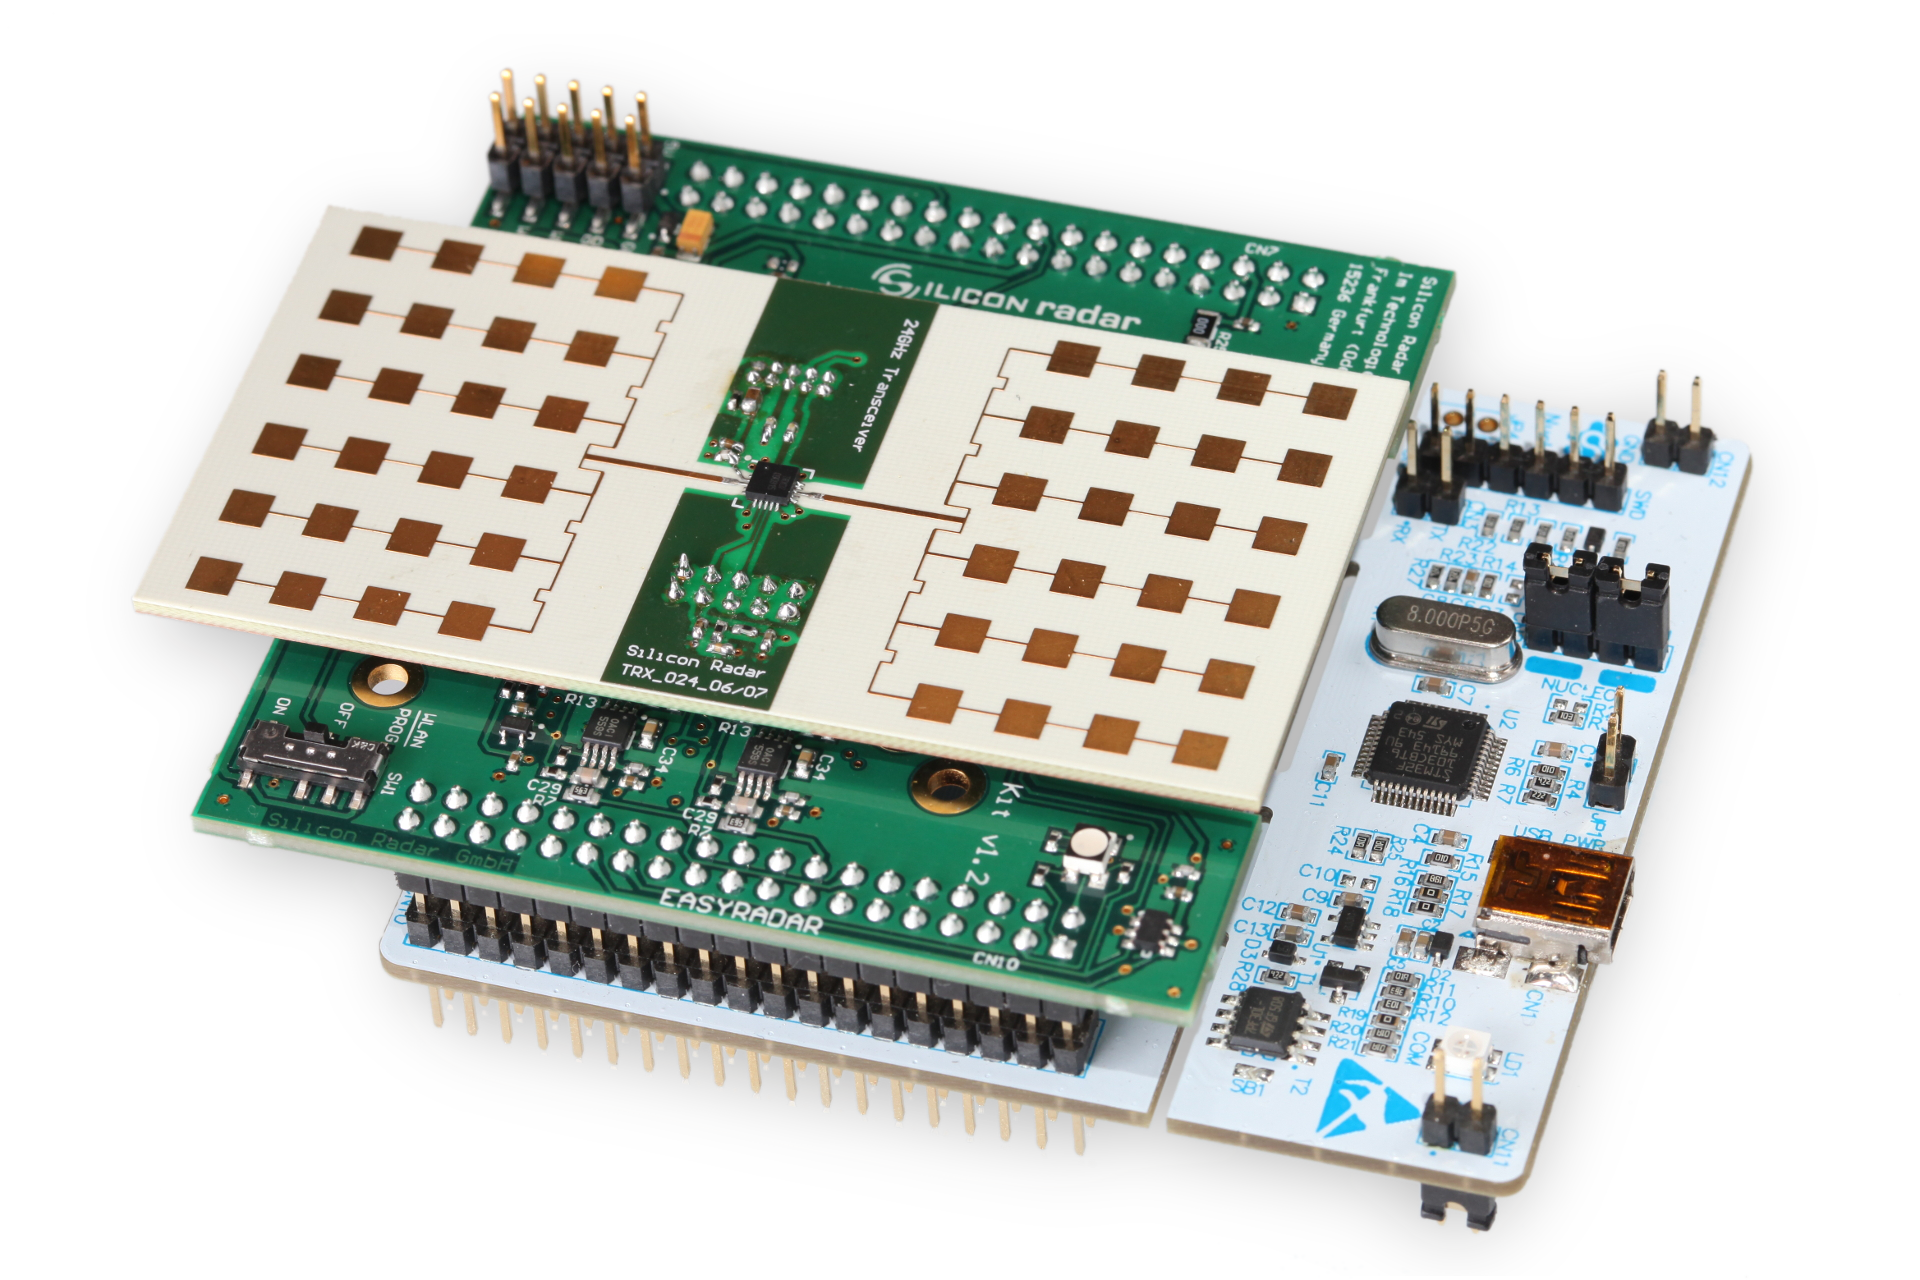
\includegraphics[width=0.7\textwidth]{../img/sidar.png}

	\caption[\sidar \cite{sidarMANOld}]{\sidar  24~GHz configuration}
	\label{fig:sidar}
\end{figure}

Communication with the radar board itself isn't possible, or at least  the communication interface is not documented.
In order to configure the radar or read its measurements user is either connected to on board ESP chip via WiFi or to STM32 Nucleo series microcontroller over UART (facilitated with mini USB 2.0 connector).
Both are relatively low bandwidth communication -- the serial maxing at baudrate of 1~000~0000.

\begin{figure}[h!]
	\centering
	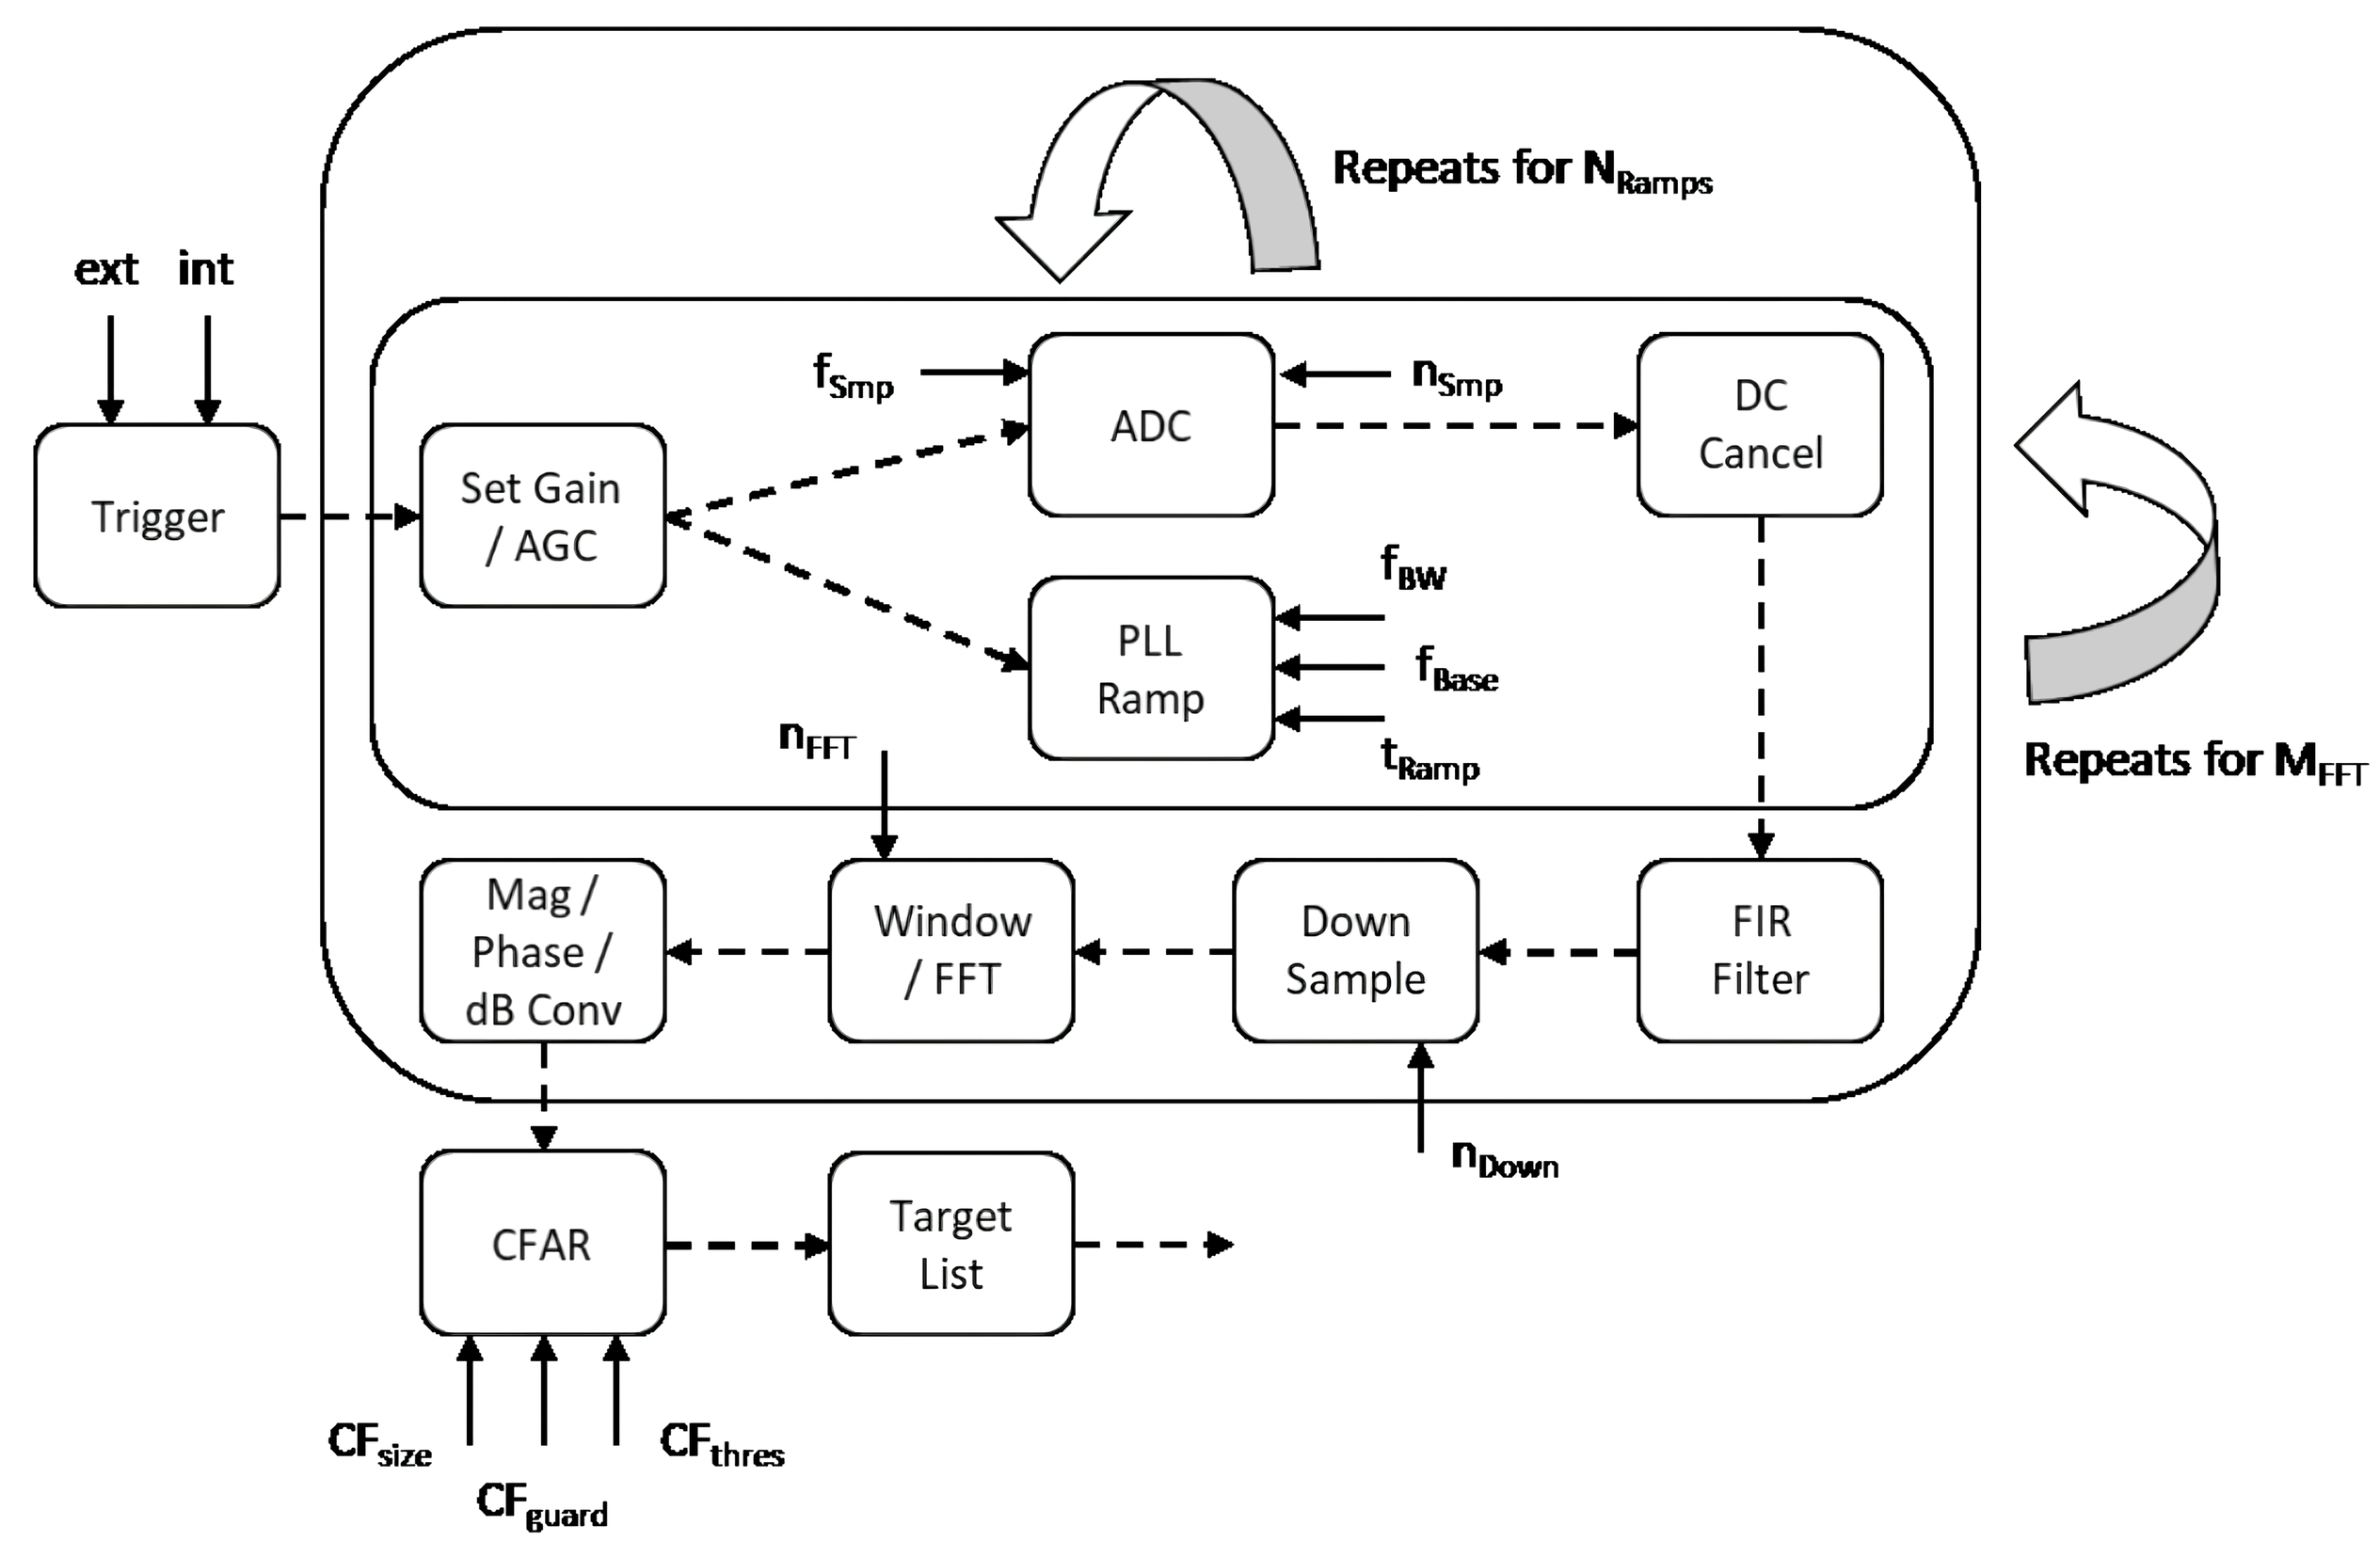
\includegraphics[width=0.7\textwidth]{../img/sidar_flow.png}
	\caption[Flow of Radar Measurement on \sidar \cite{sidarPRO}]{Flow of Radar Measurement on \sidar}
	\label{fig:sidarFlow}
\end{figure}

Devkit is designed to be as easy to integrate into existing project as possible this is unfortunately to the determent of this thesis.
In normal operating mode the radar system is a black box (Processing schema showed on \ref{fig:sidarFlow}) -- it's own filtering, FFT and CFAR algorithms and only reporting a target list to the user.

This whole sequence can be either triggered internally (driven by configurable oscillator) or externally (driven by GPIO pin or UART input).
After trigger is received the device will carry out a N chirps (or N+2 in case AGC is turned on).
Length of the chirp is derived from number or sampling steps and ADC sampling time as
\begin{equation}
	t_\mathrm{ramp} = \frac{t_\mathrm{ADC} \cdot  (N_\mathrm{samples} + 85)}{36\,\, \mathrm{MHz}} \,\, \mu\mathrm{s}
	\label{eq:sampling}
\end{equation}
with optimal time for good SNR stated to be 1~ms by the manufacturer \cite{sidarPRO}.
What is done with sampled rams hasn't been made clear by the manufacturer.
Most likely the data are somehow averaged improve SNR of the reported signal as if the  \ref{eq:sampling} is to be believed each ramp is taken with $N_\mathrm{samples}$ samples but in the end only $N_\mathrm{samples}$ are reported with their respective inphase and quadrature components.

It is worth noting that as the computational abilities of the kit are rather restrictive radar might not emit a continuos sawtooth waveform but rather a segmented one \cite{sidarPRO}.

\section{Outline of Chosen Configuration }


For purpose of this project the driver was configured to output raw data from the 12 bit ADC in form of inphase and quadrature components of the signal.
This allows for a more detailed analysis of the radar system and the possibility of implementing custom signal processing algorithms.
For these reasons default windowing was also turned off.

After configuring output regimes its necessary to pick correct balance of number of ramps, samples and sampling frequency.
As the radar will be moving there is obvious need to get reports from the radar as frequently as possible.
With faster updates we can move the platform faster and it is more possible to use neighboring samples as the angular distance between them won't be that large.

Decreasing the number of ramps slightly improves frequency of reports.
However the increase of speed is quite small -- decreasing the number of ramps from 16 to 1 only leads to 11~\% faster reporting speed.
Similarly small  gains in speed occur even when changing the sampling frequency.
Only parametr that has a large impact on frequency of reports is number of samples -- halfing the number of samples leads to some 50~\% improvement.
This is with sampling frequency adjusted for optimal SNR (close to 1~ms).
Still even then report comes in every roughly 60~ms and the maximal distance is more than halved.


Another parameter that warrants some consideration in rotary usecase is AGC.
Using it adds two additional ramps that are used solely to set gain value but it also can lead to inconsistent weights of values between two neighboring data sets.
Though the latter this is unlikely as the gain setting are quite far apart (8~dB$\Rightarrow$ 21~dB $\Rightarrow$ 43~dB as listed in \cite{sidarPRO}) so a difference in distance would have to be quite large.
Thus its safest to turn AGC off and set the gain manually depending on how the readings appear.

It's also worth to point out that the radar system isn't really suited for changing configuration on the fly.
Configuration takes a quite a long time to be applied not to mention radar doesn't provide any feedback that would enable user to send new configuration at the right time.
Thus commonly used techniques such as alternating chirp slope or frequency are not possible.

As for output format the radar system can output data in two formats -- binary and TSV.
Since the speed of output doesn't differ much between those two formats the deciding factor is speed of parsing each of them.
There even tough MATLAB isn't really suited for parsing binary data it still comes out around 40\% faster than parsing human readable TSV data.

\section{24~GHz Header}

Center of 24~GHz header is a SISO TRX-024-007 transceiver which integrates low noise amplifier, frequency mixer, filters and VCO into a single chip.
It's designed to broadcast primarily in the ISM band (24.0-24.25~GHz) additionally ultra-wide bandwidth mode is also supported (23-26~GHz) \cite{sidarTRX24} however this mode cannot be enabled on the development kit \cite{sidarPRO}.
In its main band transmitter output power is in the range of 2.5-6~dBm depending on the configuration \cite{sidarTRX24}.
Maximal range of 400~m is advertised \cite{sidarMANOld}, however this is likely under ideal conditions when observing a large target.

As showed on picture \ref{fig:sidar} the chip is connected to two microstrip patch antennas.
Patches are placed in relatively standard configuration forming a 6 by 4 array with spacing roughly equal to half of the wavelength at 24~GHz.

Since the manufacturer wouldn't provide any information about the radiation pattern of the array a simulation was carried out using CST simulation suite.
In addition substrate parameters also weren't provided by the manufacturer for the radar board specifically.
Thankfully in the TRX-024-007 datasheet there is a board stack up for the evalutions board for the chip itself.
It was assumed that same stack up would be used -- 18~$\mu$m copper for the traces and grounding plane with 250~$\mu$m thick substrate of Rogers RO4350B \cite{sidarTRX24}.

After measuring the dimensions of the array using a classical optical microscope the whole array was redrawn in CST studio.
Picture \ref{fig:boundaries} than shows a boundary conditions used -- antenna was placed in open space and alongside the symmetry plane a $H=0$ condition was set in order to speed up the simulation.

\begin{figure}[h!]
	\centering
	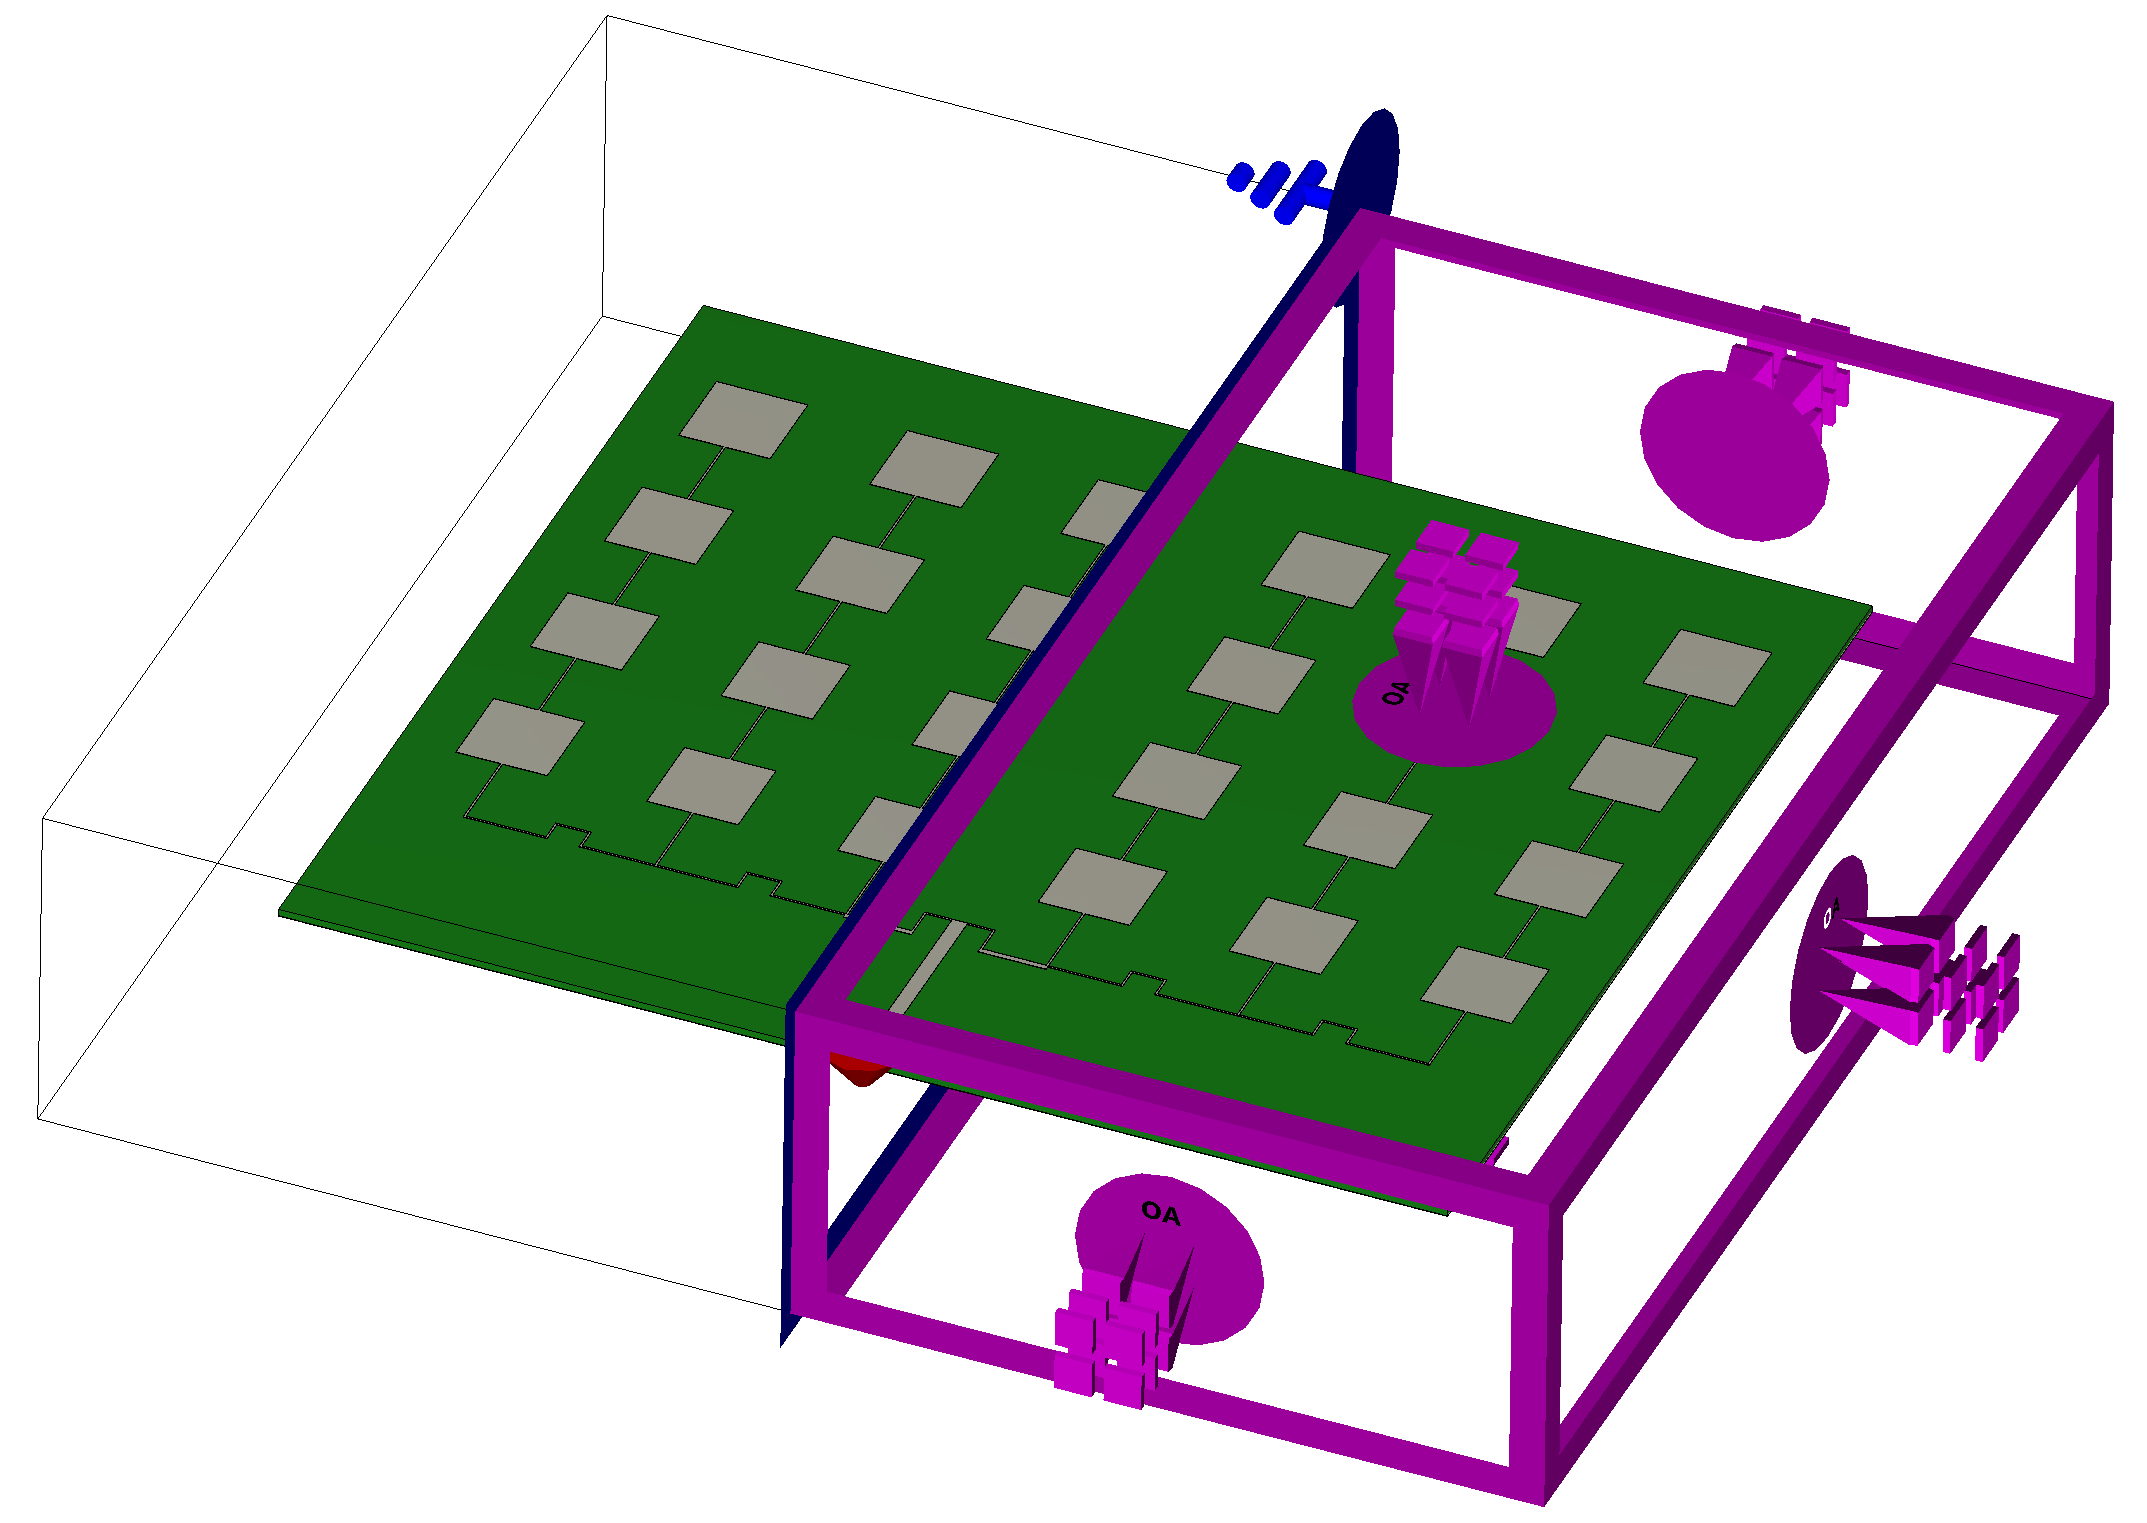
\includegraphics[width=0.7\textwidth]{../img/boundaries.png}
	\caption[Simulated 24 GHz header with boundary conditions showed]{Simulated 24 GHz header with boundary conditions showed}
	\label{fig:boundaries}
\end{figure}

\begin{figure}[h!]
	\centering
	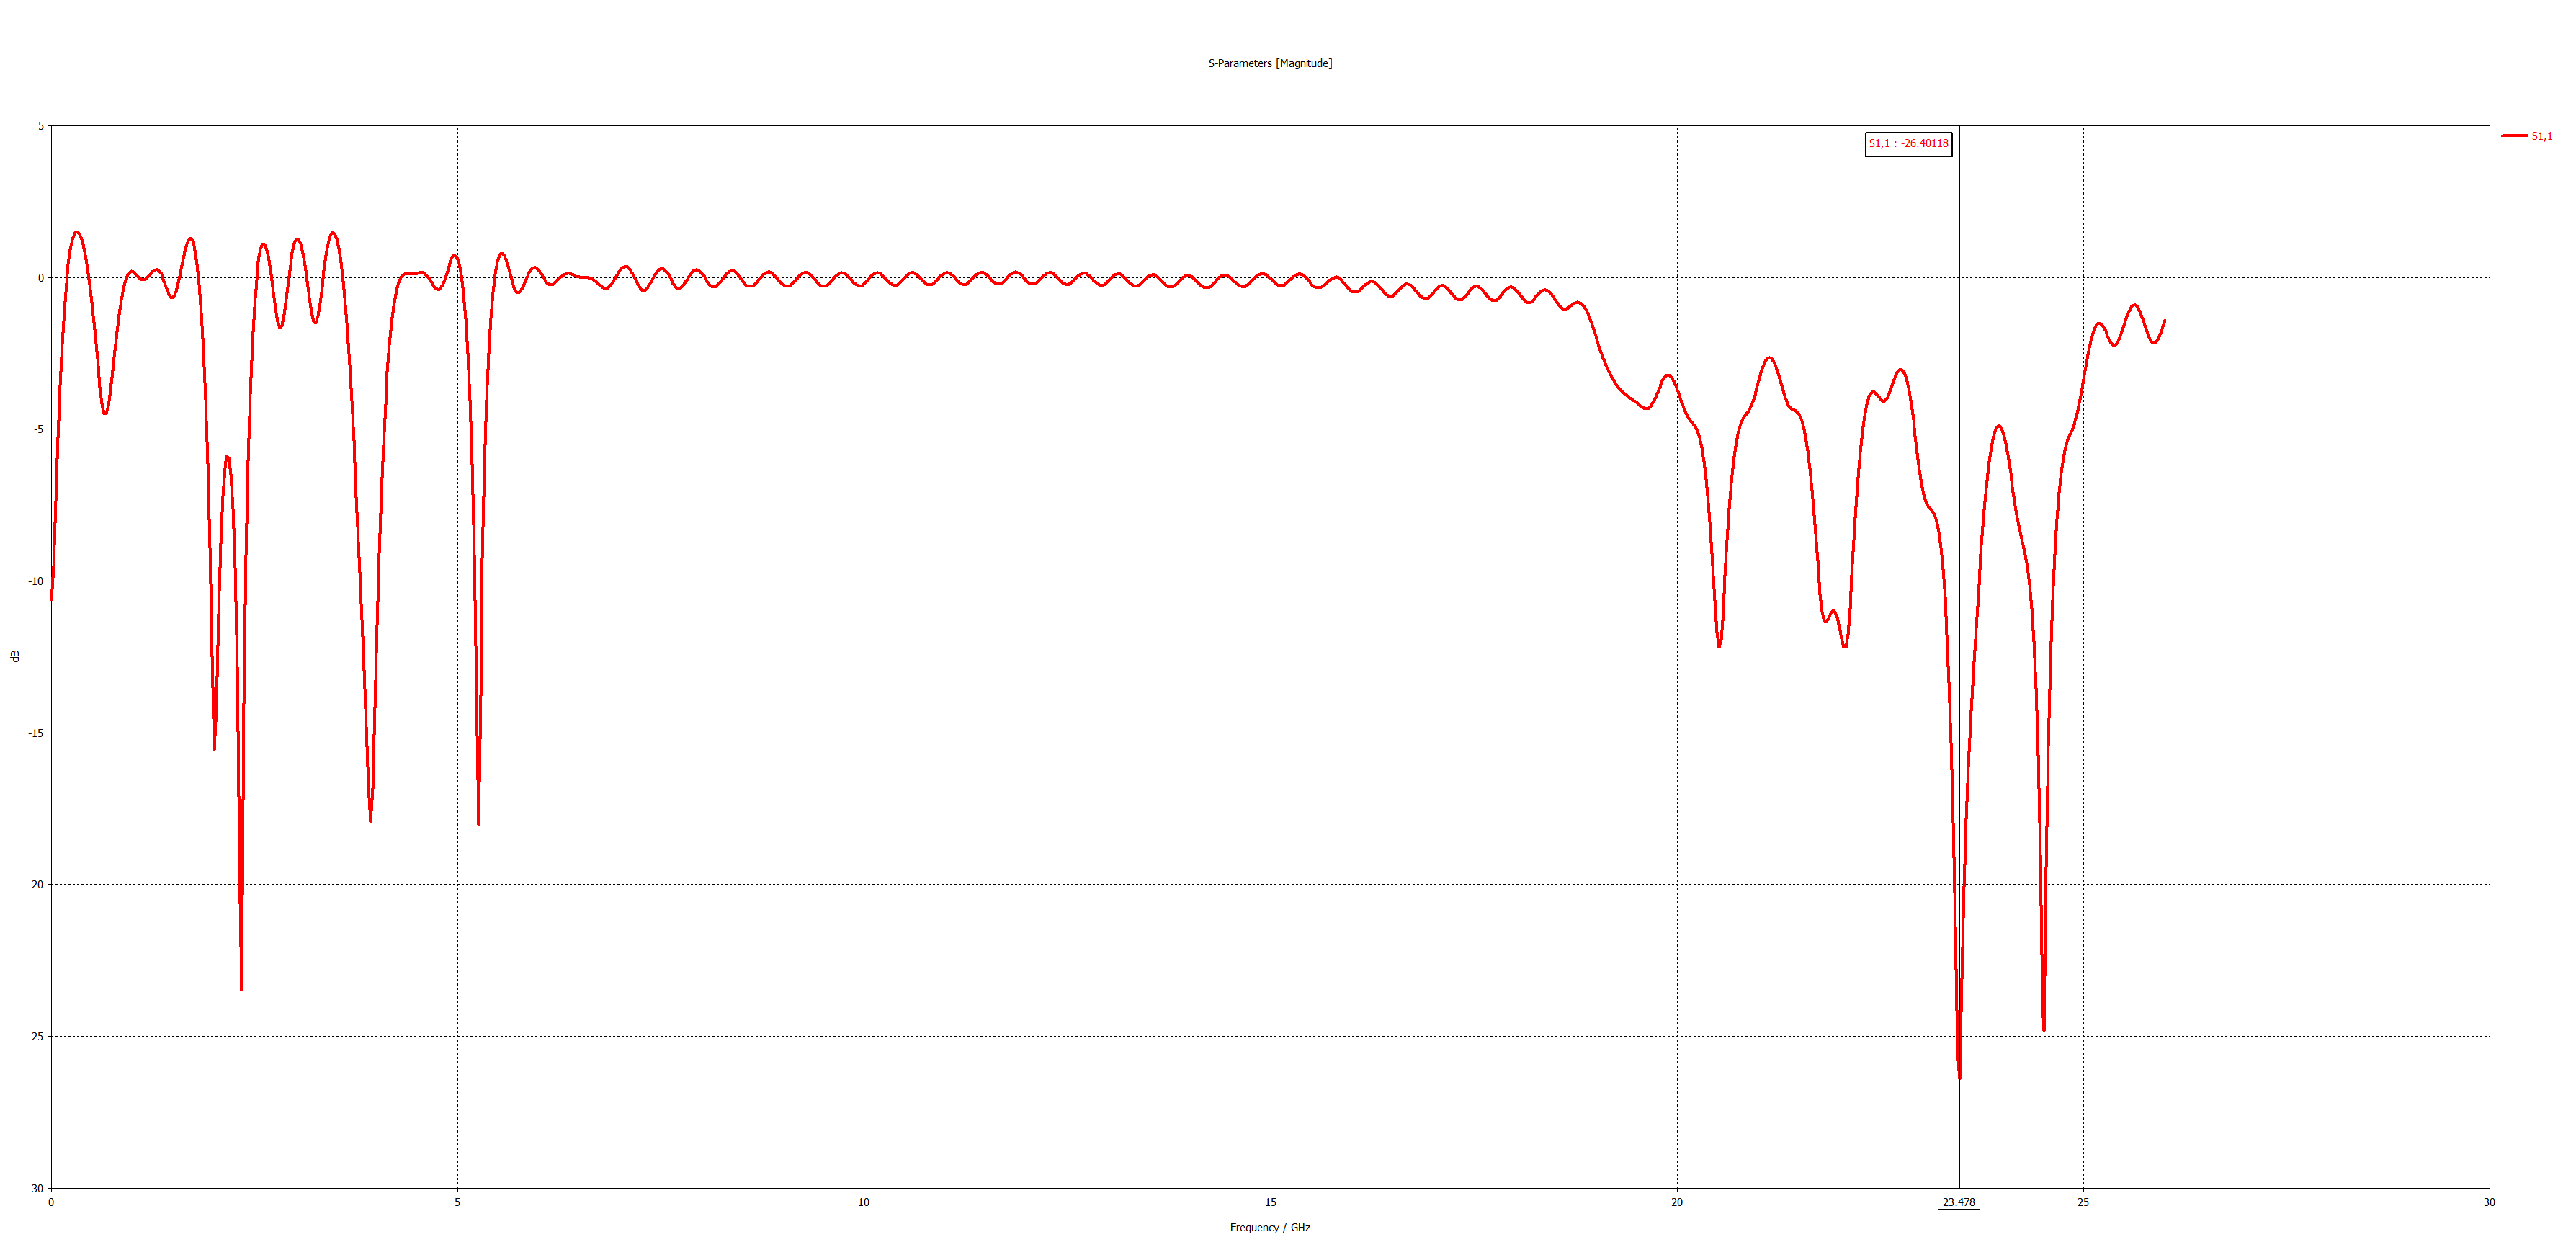
\includegraphics[width=0.9\textwidth]{../img/s11.png}
	\caption[$s_{11}$ parameter of the 24~GHz header]{$s_{11}$ parameter of the 24~GHz header}
	\label{fig:s11}
\end{figure}

After carrying out standard time simulation with excitation of the antenna with signal from 0 to 26~GHz the antenna array showed a smallest reflection coefficient $s_{11} \doteq -26.4 \mathrm{~dB}$ at 23.478~GHz with second minimum at 24.518~GHz.
This could be explained by difficulties in measuring exact dimensions (Etching quality of the copper tracer wasn't the greatest.) and neglecting change of substrate parameters due to interactions of different layers.

At both frequencies with minimal reflection a farfield radiation pattern was calculated for the sake of clarity only the 24.518~GHz one is shown in \ref{fig:farfield3d}.
Main lobe width was measured at roughly 16 degrees \ref{fig:farfield180} at 180 degrees norm (for orientation use red cone on the PCB) at 18.6~dBi gain and -12~dB side lobe suppression.
For 90 degree norm the main lobe width \ref{fig:farfield90}was 30 degrees with -10~dB side lobe suppression.

\begin{figure}[h!]
	\centering
	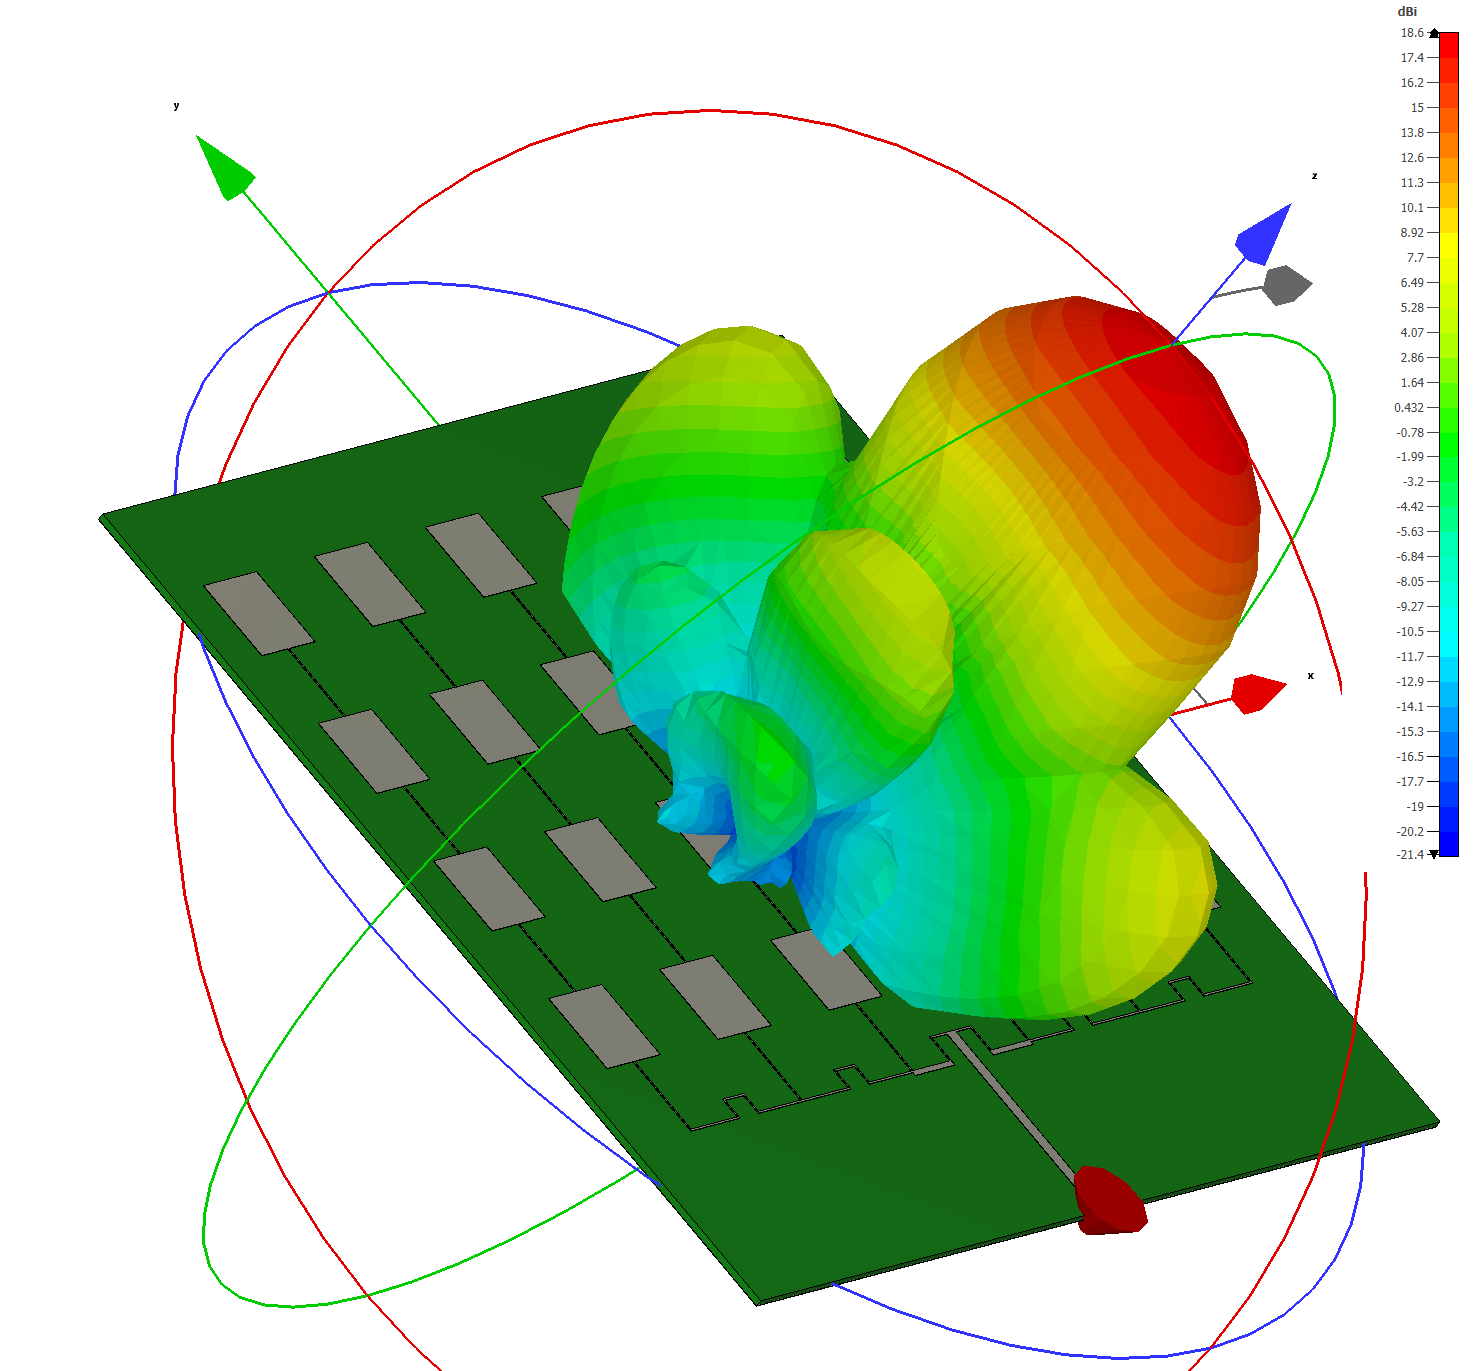
\includegraphics[width=0.7\textwidth]{../img/farfield3d.png}
	\caption[Radiation pattern of 24~GHz header -- 3D view]{Radiation pattern of 24~GHz header -- 3D view}
	\label{fig:farfield3d}
\end{figure}

\begin{figure}[h!]
	\centering
	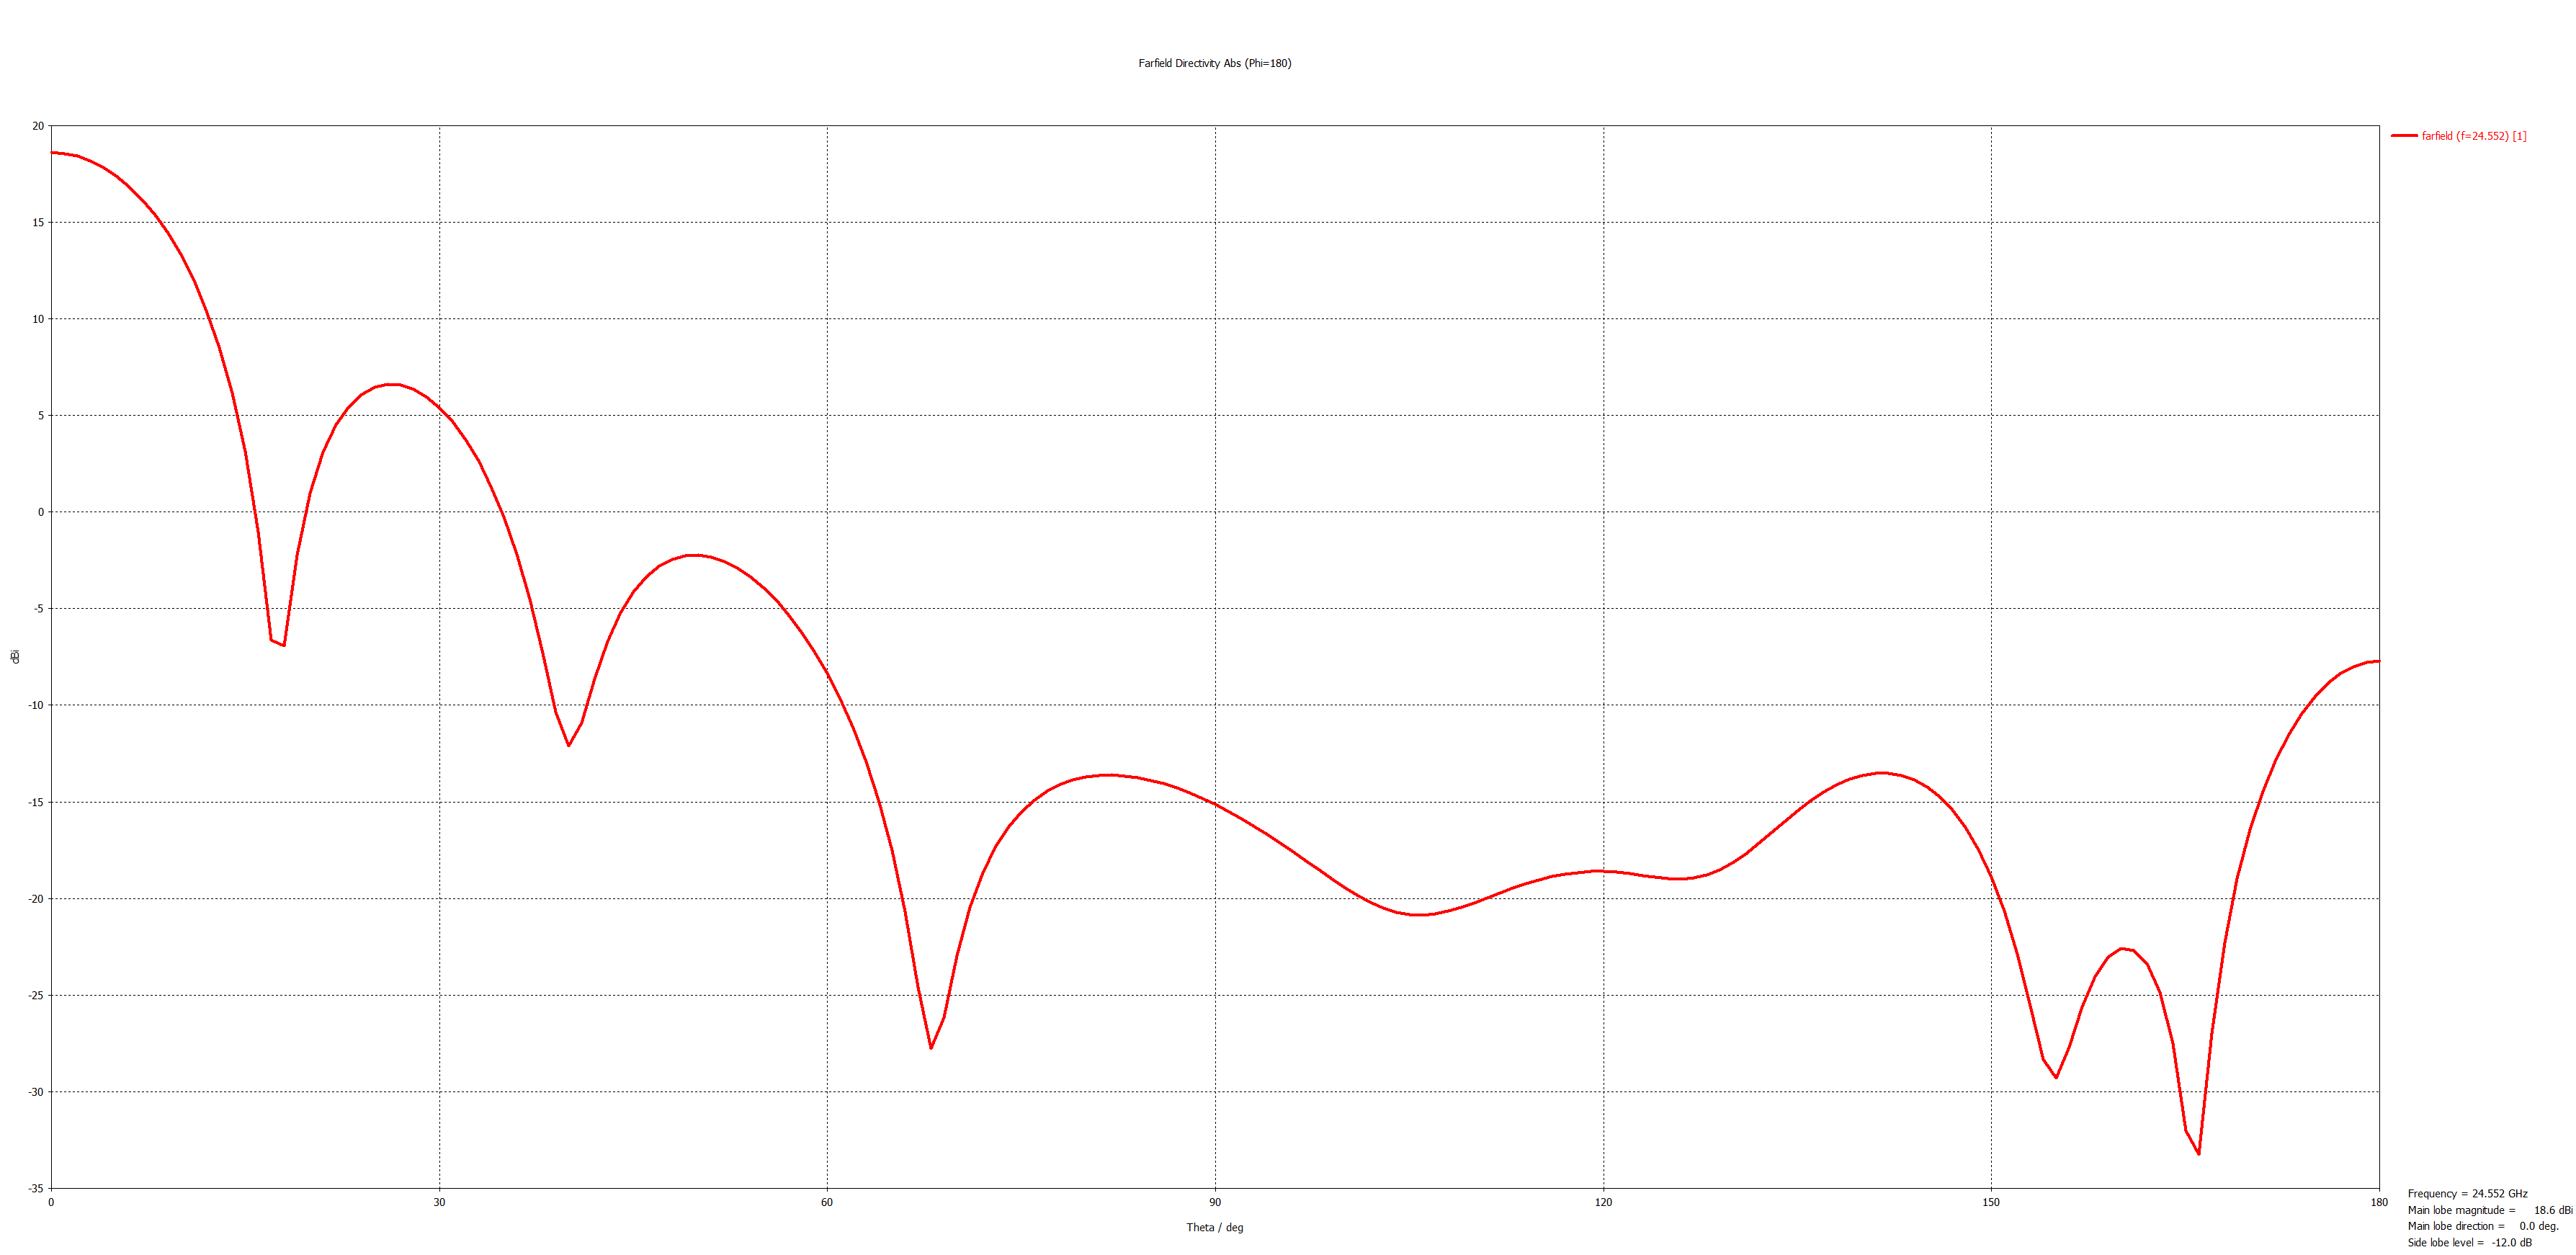
\includegraphics[width=0.7\textwidth]{../img/farfield180.png}
	\caption[Radiation pattern of 24~GHz header -- 180° norm]{Radiation pattern of 24~GHz header -- 180° norm}
	\label{fig:farfield180}
\end{figure}

\begin{figure}[h!]
	\centering
	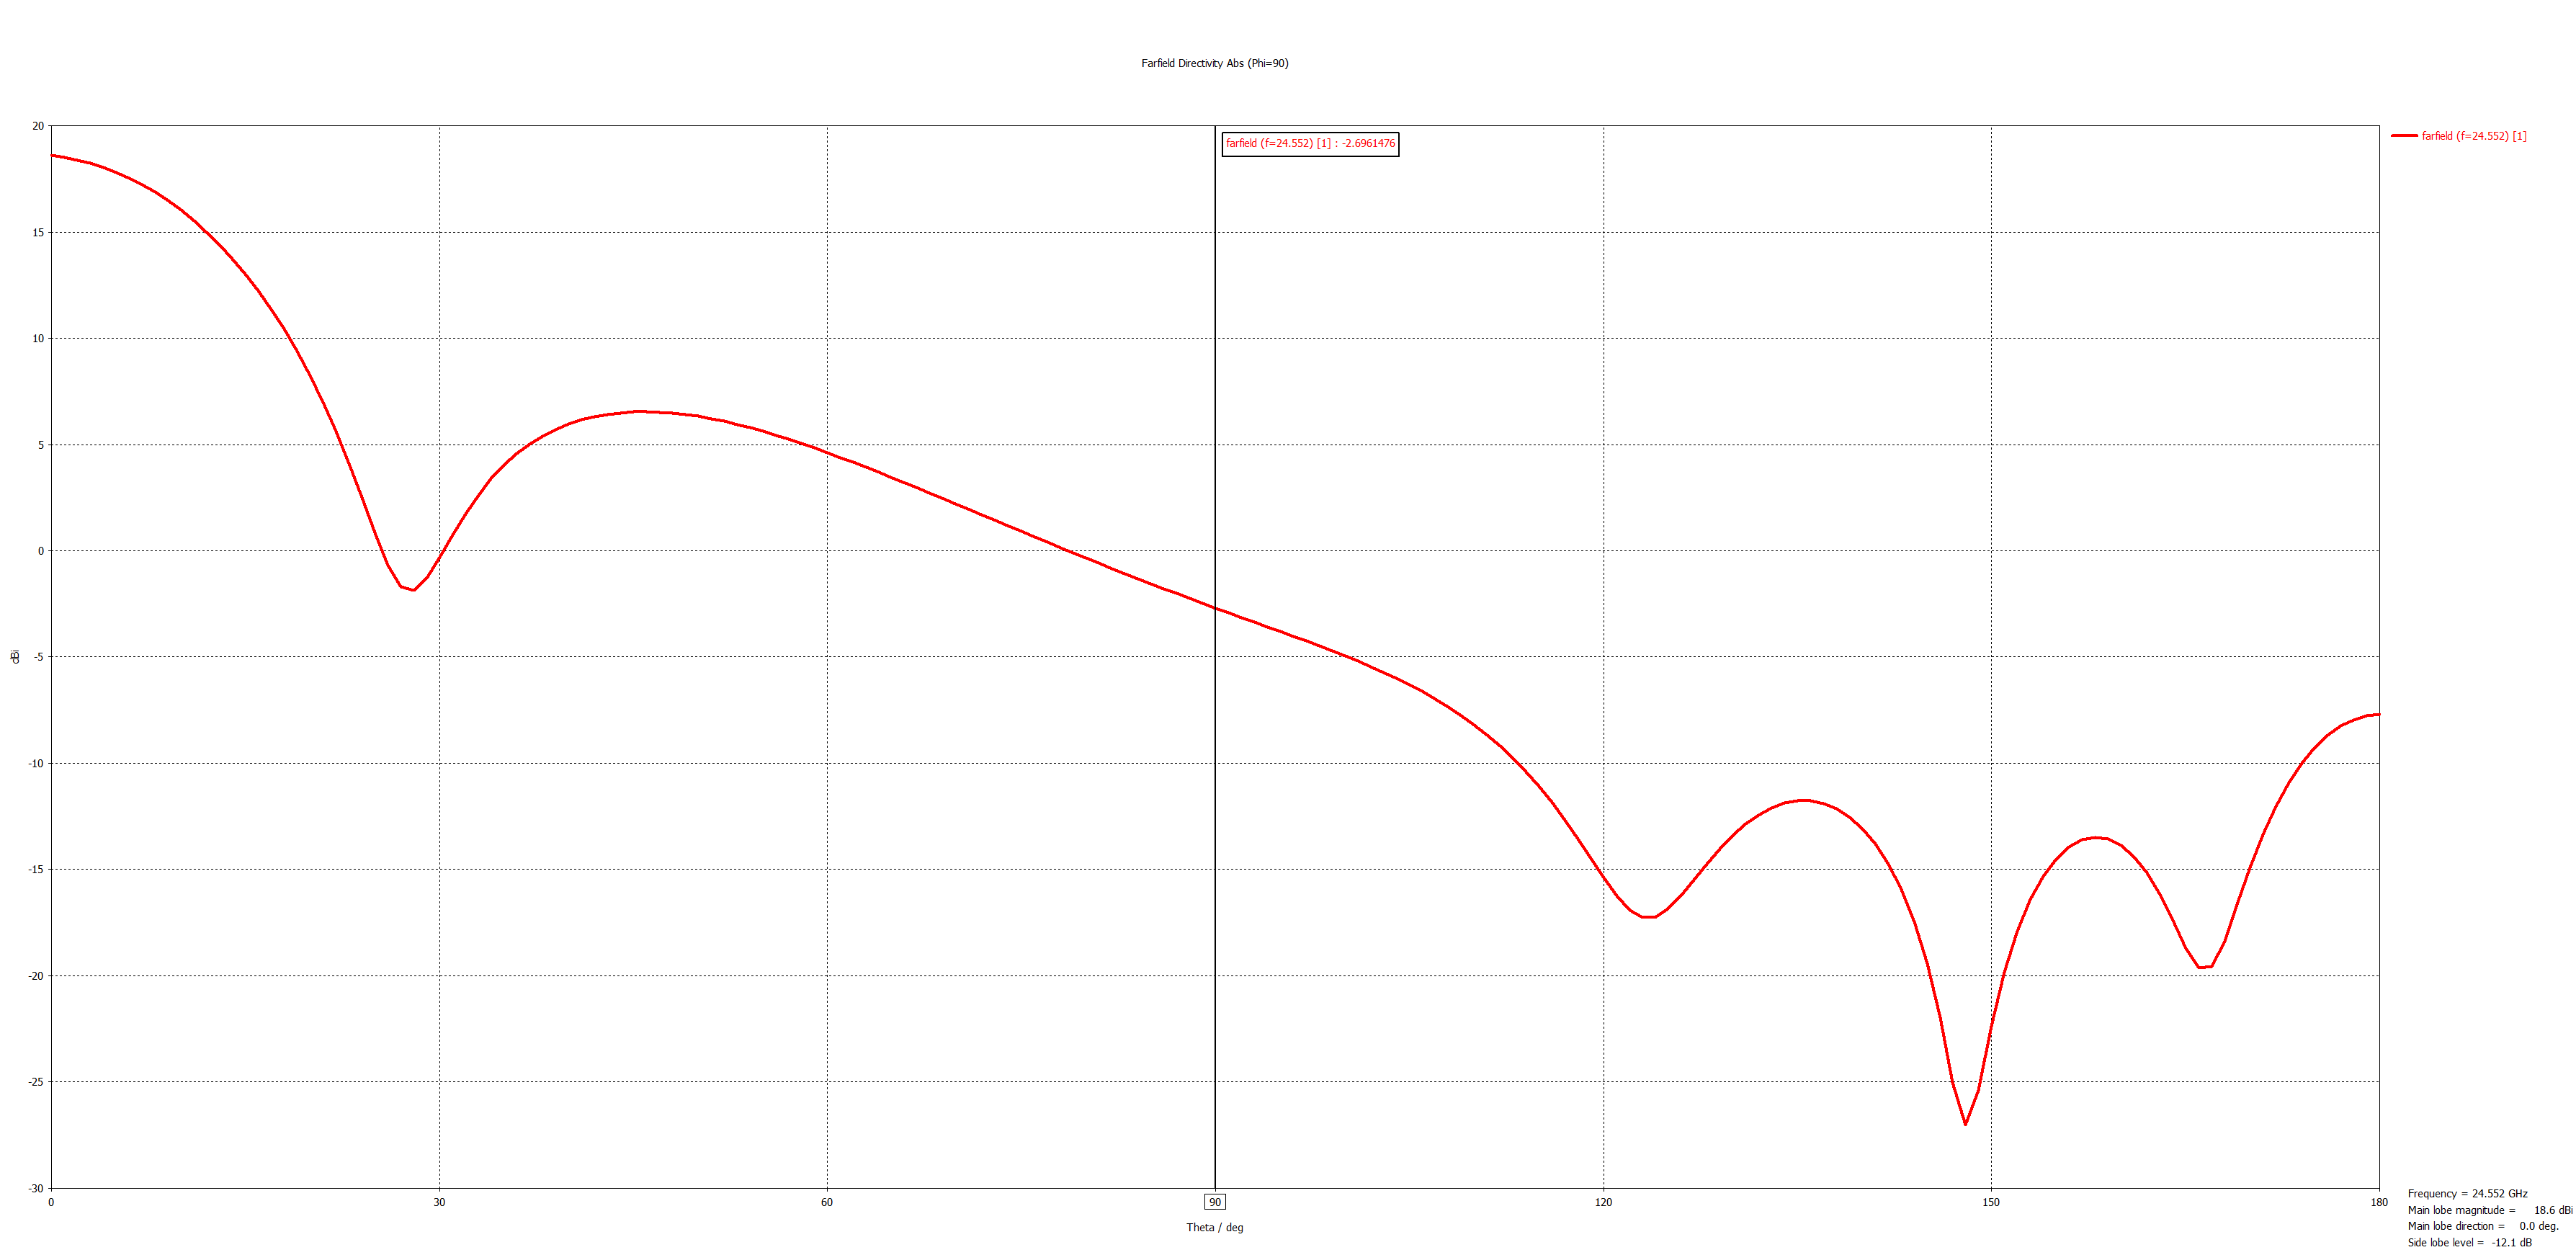
\includegraphics[width=0.7\textwidth]{../img/farfield90.png}
	\caption[Radiation pattern of 24~GHz header -- 90° norm]{Radiation pattern of 24~GHz header -- 90° norm}
	\label{fig:farfield90}
\end{figure}


\section{122~GHz Header}

\begin{figure}[h!]
	\centering
	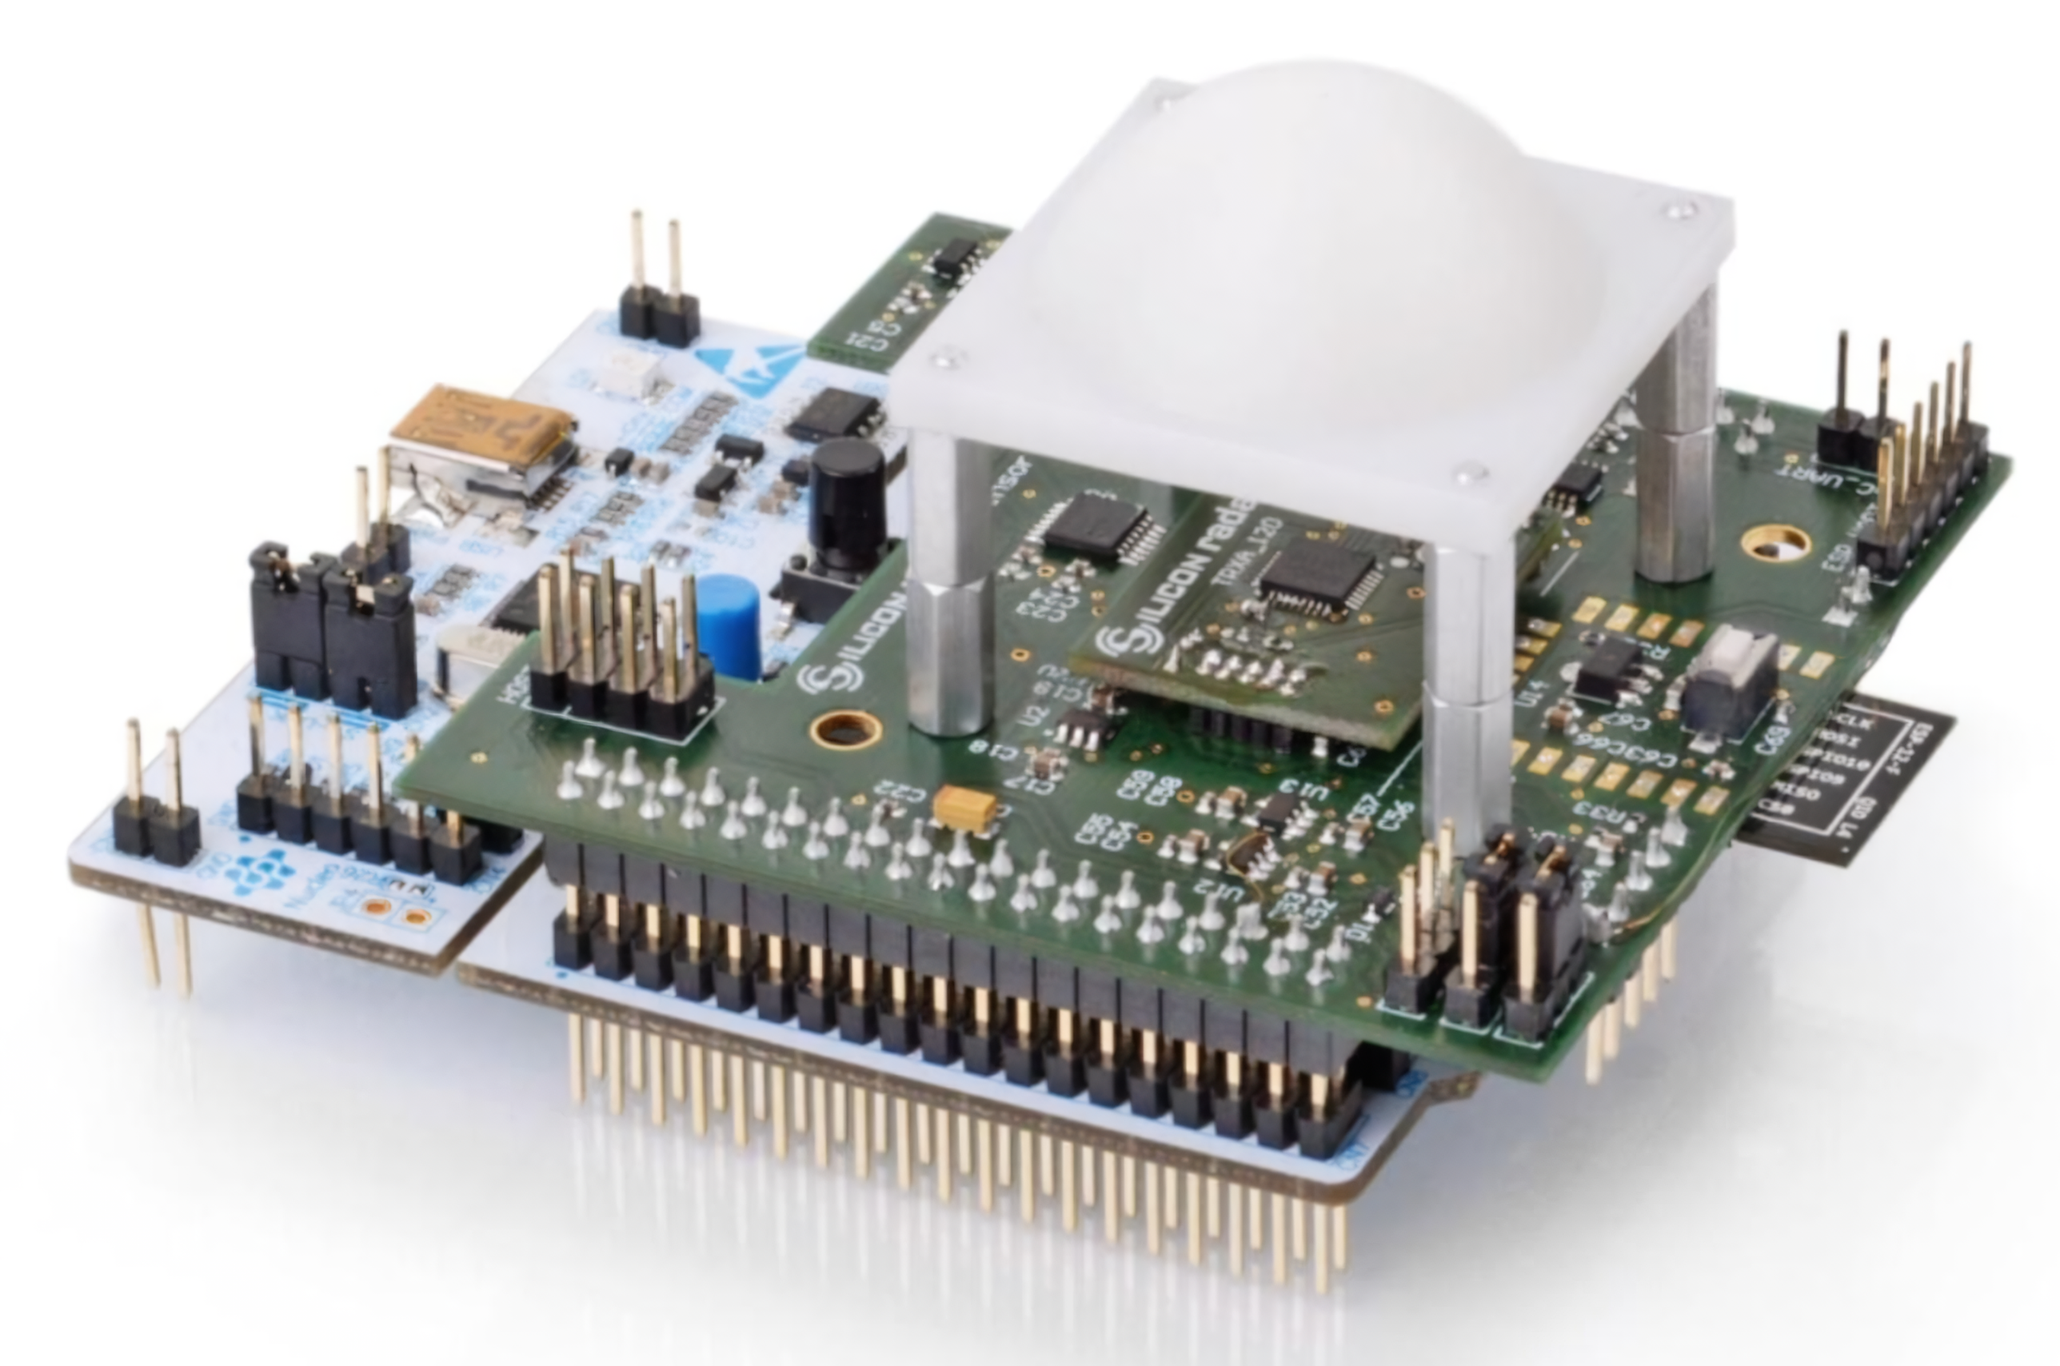
\includegraphics[width=0.7\textwidth]{../img/sidar122.png}
	\caption[\sidar with 122~GHz header \cite{sidarPRO}]{\sidar with 122~GHz header}
	\label{fig:sidar122}
\end{figure}

\begin{figure}[h!]
	\centering
	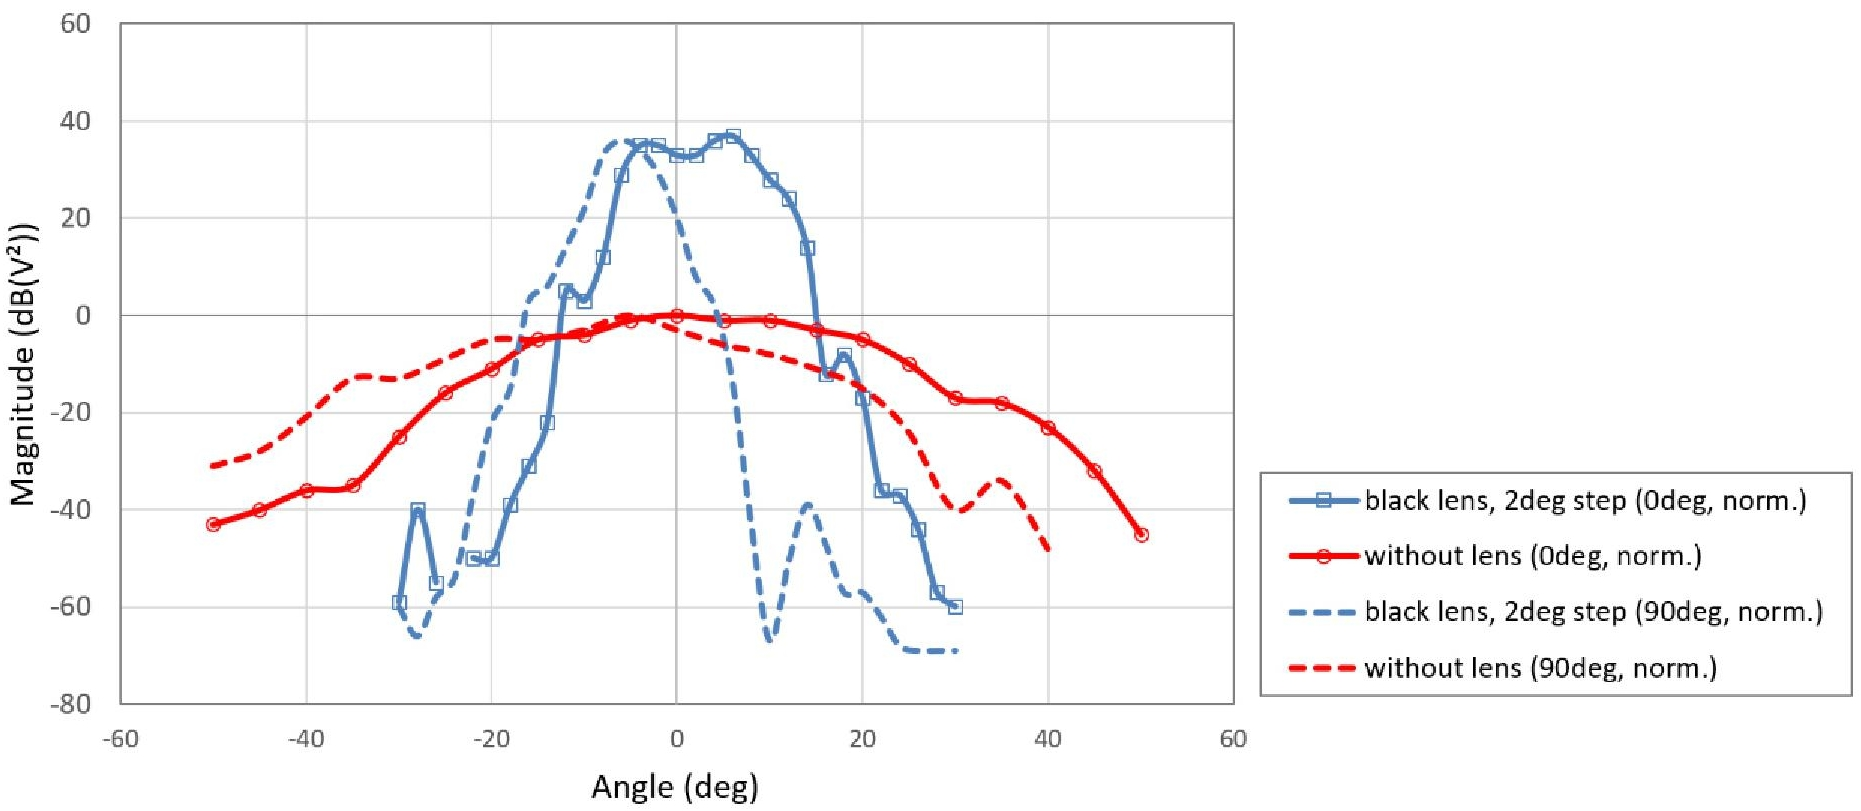
\includegraphics[width=0.7\textwidth]{../img/sidar122rad.jpg}
	\caption[Radiation pattern of 122~GHz header comparison \cite{sidarTRX122col}]{Radiation pattern of 122~GHz header comparison}
	\label{fig:sidar122rad}
\end{figure}

122~GHz header is based on TRX-120-001 transceiver which, aside from basic components needed to transmit and receive RF, also incorporates two on-chip antennas.
It's designed to operate in the 122-123~GHz band and with output power ranging from -7~dBm to 1~dBm \cite{sidarTRX122}.
Out of the box performance of the system is quite bad (see \ref{fig:sidar122rad}) with width of the main lobe being roughly $\pm40\text{°}$ in both E-plane and H-plane \cite{sidarTRX122}.
This can be improved by supplied collimator lens to $\pm4\text{°}$ \cite{sidarTRX122col} (see \ref{fig:sidar122rad}).
The chip can detect large targets up to 40~m away \cite{sidarMANOld}.




\chapter{Rotary Platform}

Following chapter outlines design process and operation of a rotary platform specifically designed for \sidar radar system.

\section{Platform Design Parameters}


To begin, it is essential to outline the fundamental requirements for the platform.
These stem from the physical capabilities of the radar system, SiRad Easy evalutions kit, and requirements for the software.

\subsection{Physical Capabilities}

The primary constraints on the physical design arise from the radar's radiation pattern (Both 24 and 122 GHz headers are accounted for.).
That gives us information about the clearance needed in front of the radar and more importantly how precise the platform needs to be.
As stated previously the 24~GHz radar has a main lobe width of some $\pm7\text{°}$ and the 122~GHz radar has a main lobe width of $\pm4\text{°}$ \cite{sidarTRX122}.
Thus a conservative clearance of $\pm45\text{°}$ in front of the radar was set in order to prevent any strong reflections be it from the main lobe or side lobes.

With a relatively low angular resolution of the radar a high precision of the platform is not needed.
Basic 200 step stepper motor with step size of 1.8\text{°} is sufficient however smoother motion will be easier to compensate for in the software.
Still due to low radar weight, measured at 120~g with the mounting bracket, the smoothens of the motion can be achieved relying solely on microstepping of the motor.

In terms of speed high-speed movement is unnecessary.
The manufacturer specifies a maximum update frequency of 50 Hz, equating to a new update every 20 ms \cite{sidarMAN}.
And in this application the update frequency will be closer to 10 to 20 Hz.
Using the following equation:
%
\begin{equation}
  t_{\mathrm{angle}} = \frac{60}{360\cdot N_{\mathrm{RMP}}} \cdot  \alpha,
  \label{eq:poll}
\end{equation}
%
where $t_{\mathrm{angle}}$ is time between spend on traveling angle of $\alpha $ in seconds and $N_{\mathrm{RMP}}$ is number of rotations per minute, we can calculate that even for low RPM of 60 an angle of 8 degrees the platform travels (angular width of main lobe for 122 GHz radar) in 10 ms -- too fast to properly interpret the data.


\subsection{Software Requirements}

Given its widespread adoption as an industry standard for controlling multi-axis machines, G-code over serial is a natural choice for the platform's communication format. Beyond the basic functionality typically offered by G-code interpreters, the platform must support additional features to reduce the user's manual control burden. These features include the ability to define movement limits and preprogram sequences of movements for autonomous execution by the platform.

For uplink communication, the platform must provide real-time information about its current position and speed. This data allows the user to make mathematical corrections to the radar's gathered data.


\section{Platform Construction}

As the platform needs to transmit data from the rotating part to the stationary a slip ring is needed.
Due to relatively low transmission speed of the radar and lack of any special requirements, like waterproofing, an affordable model UH3899-01-0810 from manufacturer Senring was chosen classical contact slip ring was chosen.
It boasts dedicated USB 2.0 connection and 8 wires for additional signal with advertised insertion loss of sub 2~dB \cite{slipring}.

Unfortunately the manufacturer went with non standard male-male USB 2.0 connection which requires a female-female adapter in order to connect the radar to the slip ring.
Still especially when used with a poor quality cable the whole system starts to have signal integrity problems.
These issues could most likely be mitigated by integrating a signal conditioner into the transmission line.

The rest of the design is rather simple.
Fixed section mounts a slipring with stepper motor underneath directly driving a shaft connected to the rotating platform.
Connection is done using long set M4 crews that go trough the slipring and fix the shaft in place.
3D printed housing than acts only as a centering guide and isn't load bearing.

Rotating section than has a simple A frame design that elevates the radar which is mounted with bearing enabling the radar to tilt freely.
In order to control the tilt a second stepper is mounted on the rotating platform a linked with 2:1 down gearing ration using a standard 8~mm belt to the radar.
On second support start there is an optical endstop mounted that is used to home the platform.

Since mechanical stresses are quite low most parts could be 3D printed using standard PLA filament.

The rest of the structure is 3D printed from PLA, since mechanical stresses on the platform are minimal.
Only non 3D printed parts are the screws, bearings, and the stepper motors.
Final assembly \ref{fig:side_by_side} measures some 33~cm and has footprint of 20x20~cm.


\begin{figure}[h!]
  \centering
  \begin{subfigure}[b]{0.45\textwidth}
    \centering
    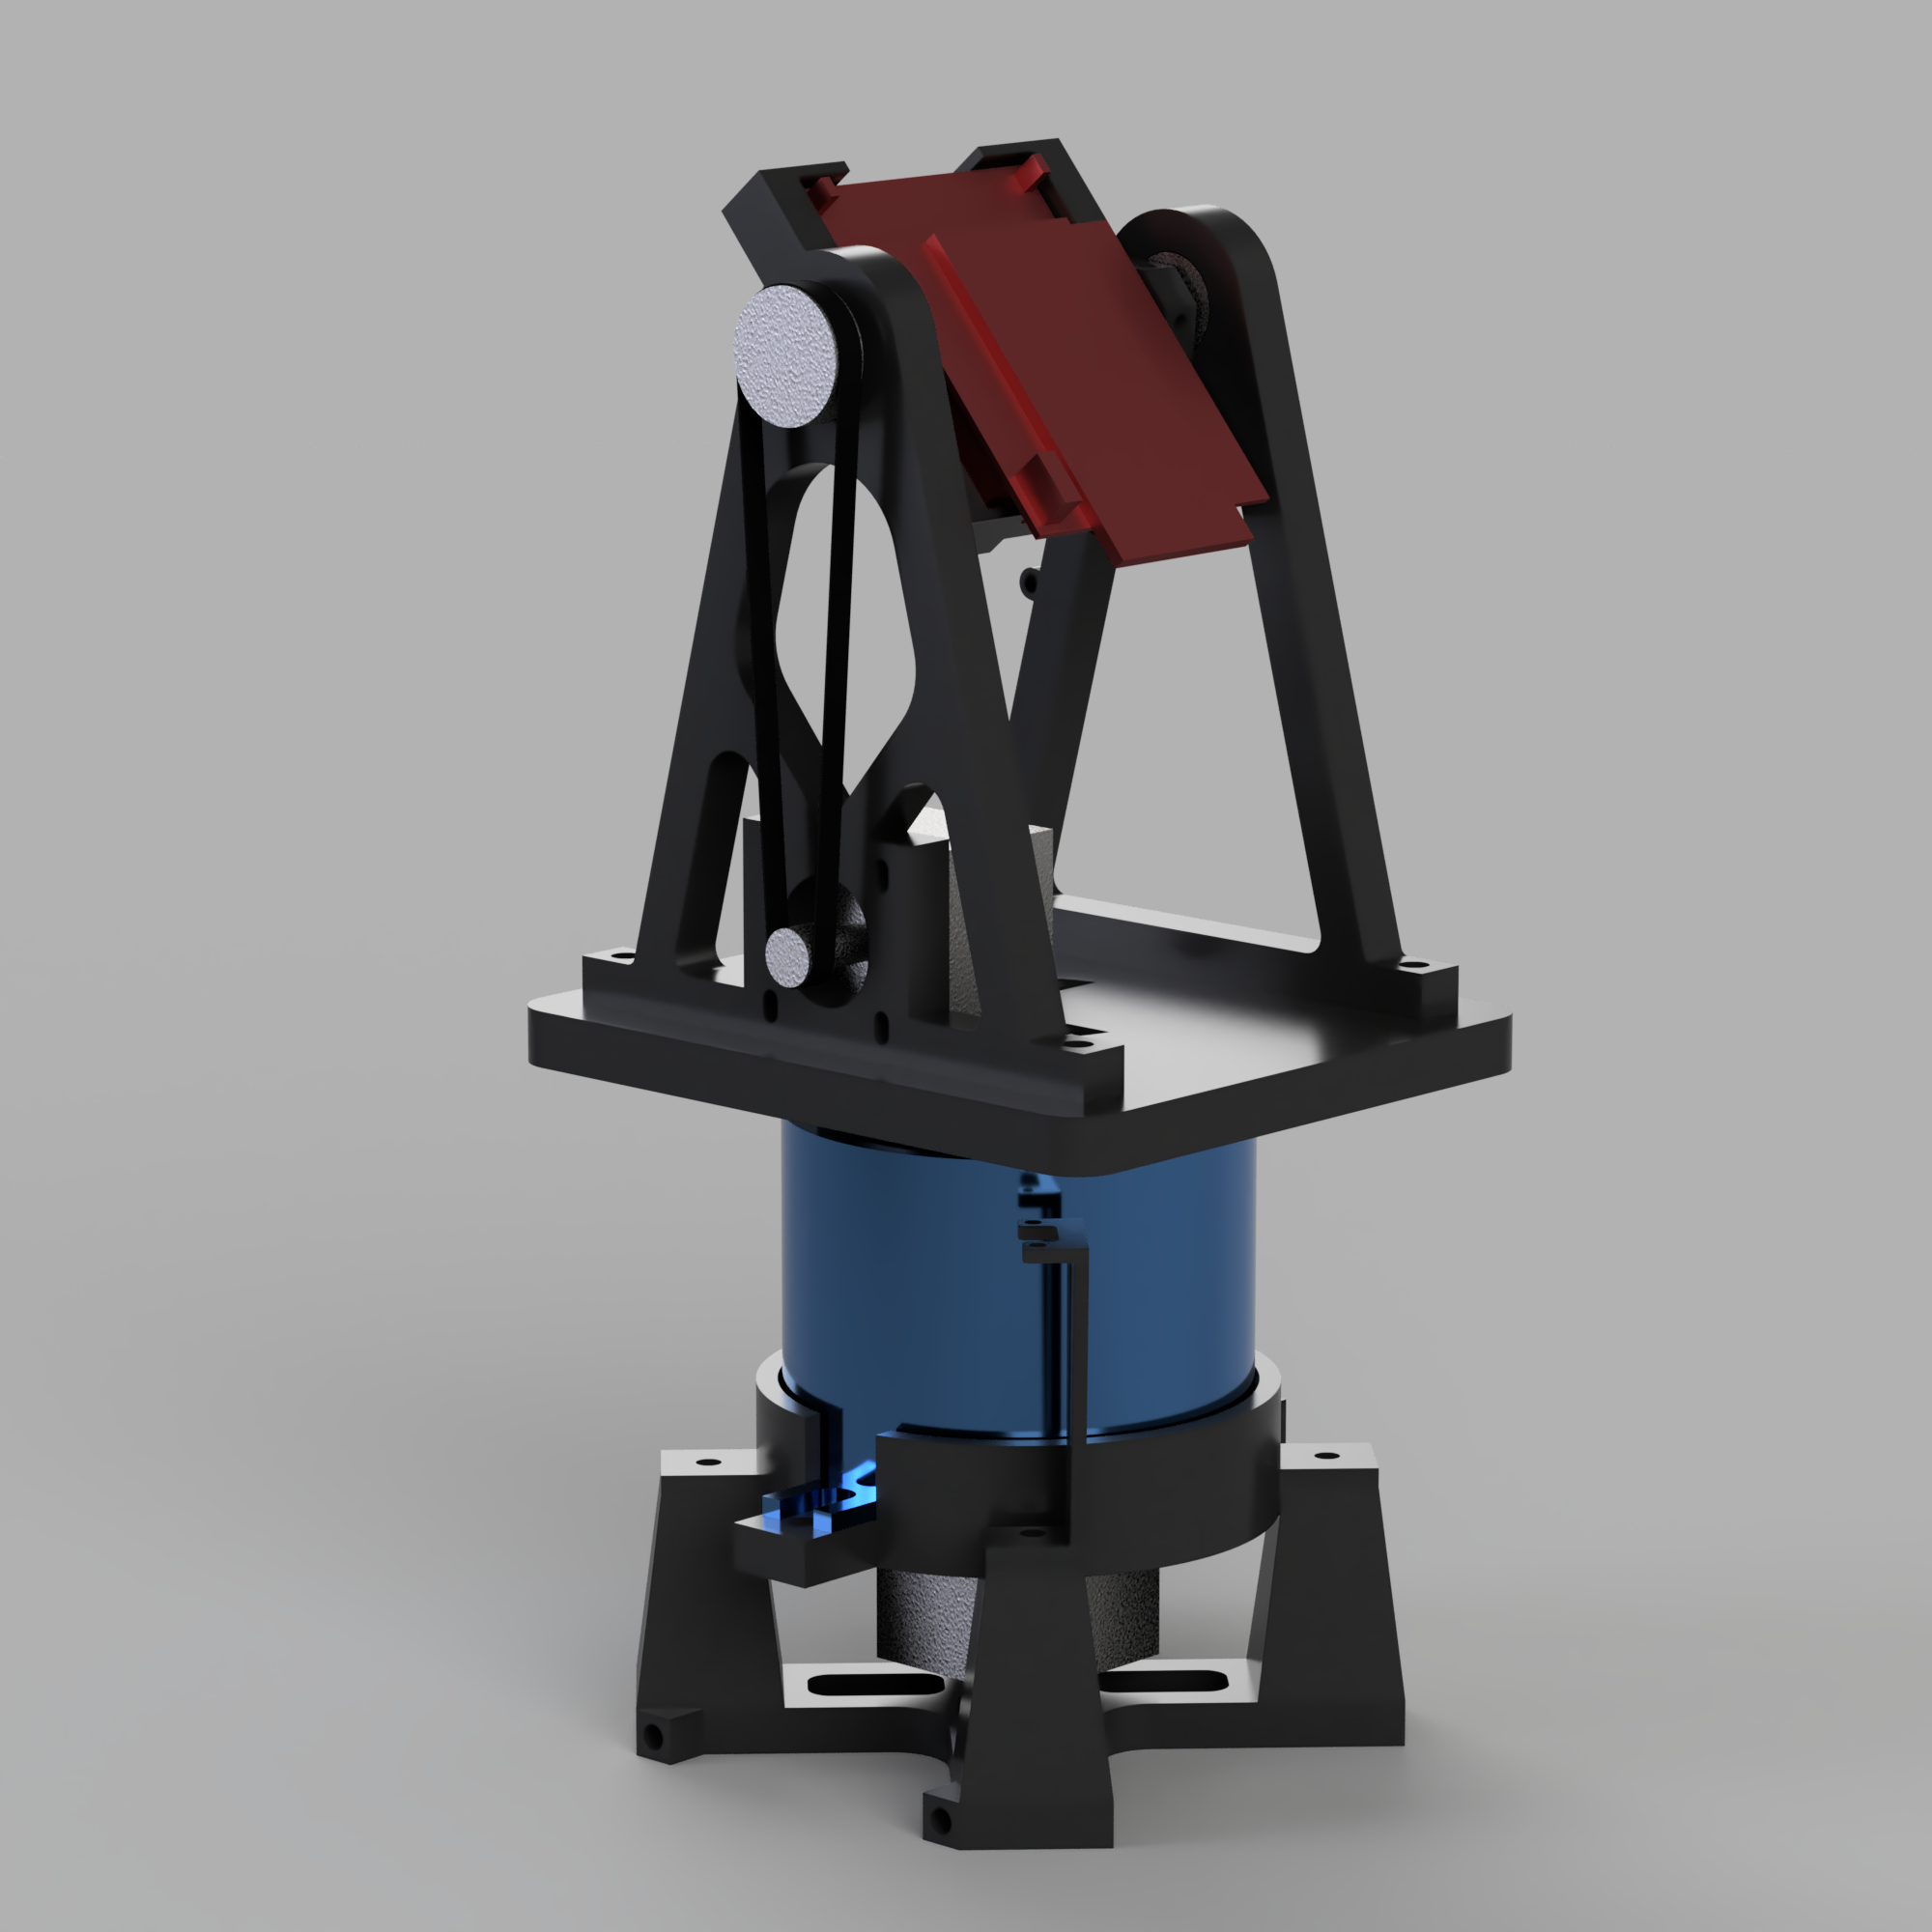
\includegraphics[width=\textwidth]{../img/whole_assembly_2.png} % Replace with your image path
    \caption{3D render}
  \end{subfigure}
  \hspace{0.05\textwidth} % Adjust spacing
  \begin{subfigure}[b]{0.45\textwidth}
    \centering
    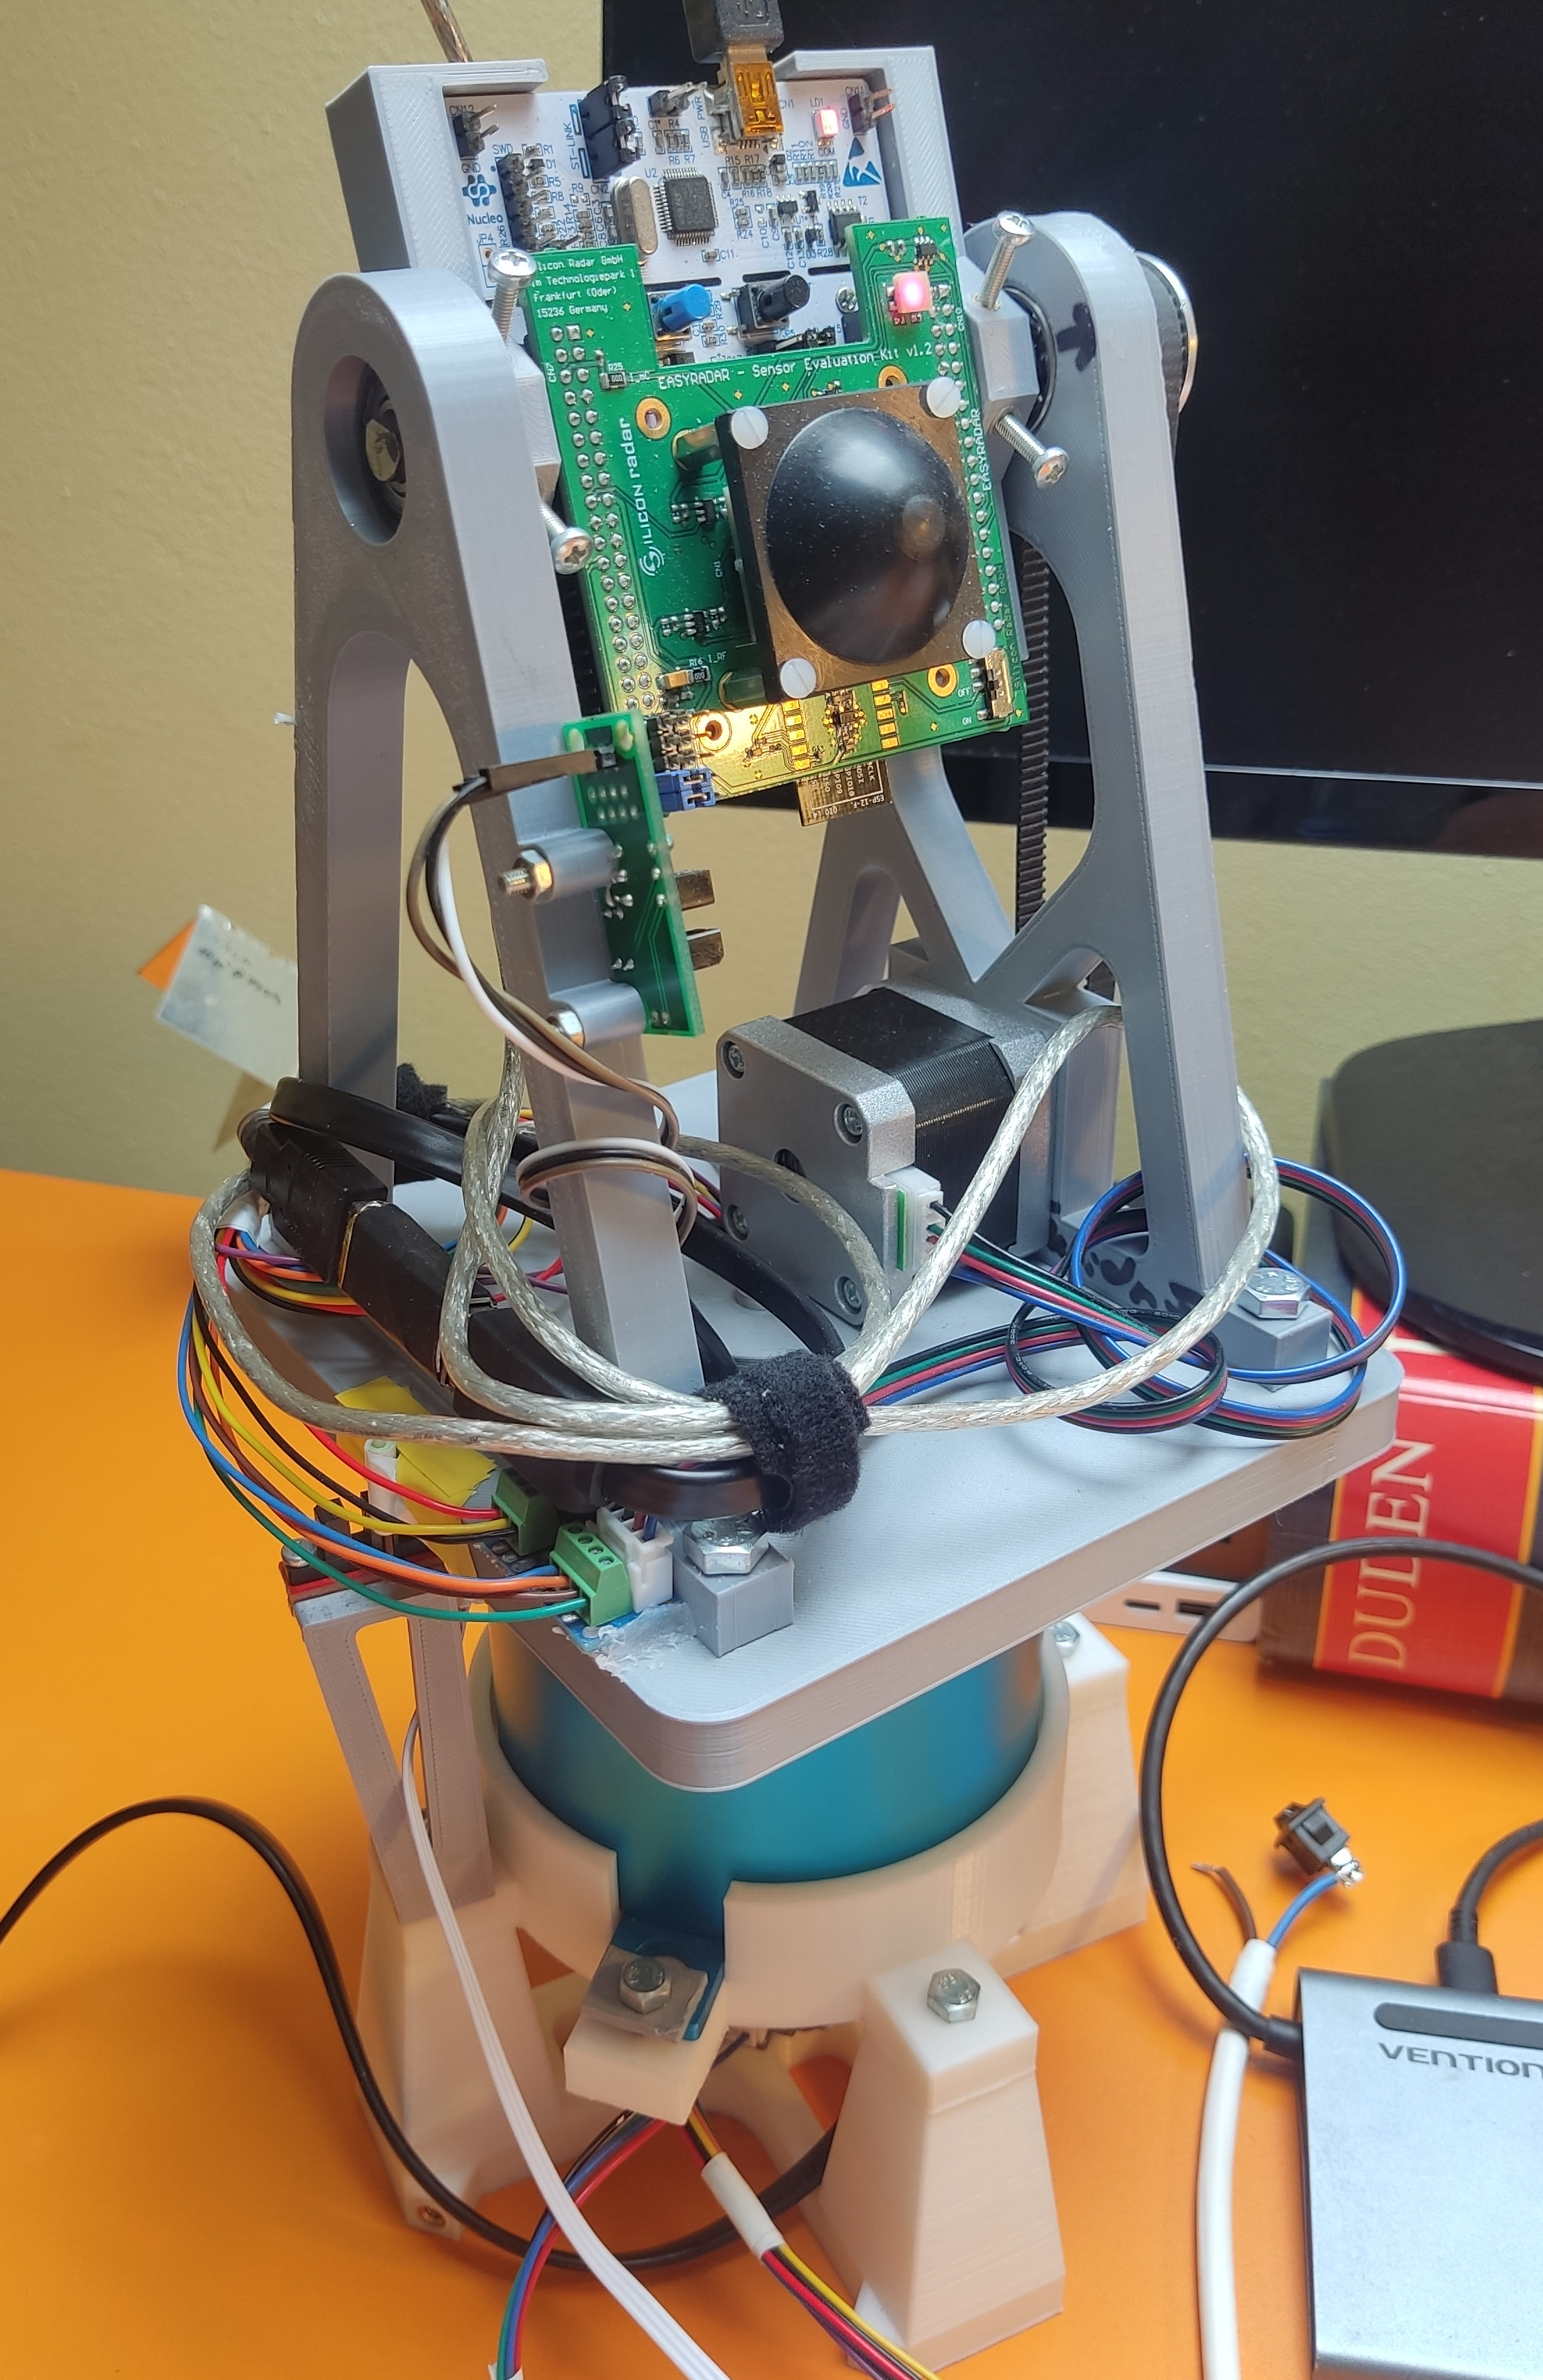
\includegraphics[width=0.75\textwidth]{../img/assembly_photo.jpg} % Replace with your image path
    \caption{Photo}
  \end{subfigure}
  \caption{Form of the final assembly}
  \label{fig:side_by_side}
\end{figure}


\subsection{Platform Electronics}

Electronic side of the project is rather simple -- there are only two things to handle: driving of stepper motors and enabling some homing mechanism.

Given the low load on stepper motors and the platform's inability to accumulate significant momentum, a simple stepper driver without feedback control is adequate.
For this purpose, the A4988 stepper driver was selected, due to its low cost, microstepping capabilities and basic current control \cite{a4988}.
Minor disadvantages is the lack of any feedback from the driver to microcontroller including some sort of stall detection.
In order to simplify the design A4988 devkits were used soldered onto a prototyping board without creating a custom PCB design.

To implement homing, two potential solutions were considered: Hall effect sensors and optical gates.
While Hall effect sensors offer the advantage of angle sensing, allowing correction of any positional drift during operation, they require precise alignment.
If the orthogonal Hall effect sensor is not perfectly placed in the axis of rotation, calibration becomes a necessity \cite{hall}.
While the feedback would be nice, given the fact that microcontroller sends signal for each step taken by the motor in normal operating conditions the position of the platform can be easily calculated using software.

Thus for simplicity and ease of integration, optical gates were selected.
This decision eliminates the need for complex calibration while providing reliable functionality.

Driving the whole system is an ESP32 microcontroller.
ESP32C6 version was chosen due to author's extensive experience with this particular version.
System doesn't require any special peripherals or high processing power thus any ESP32 version would be sufficient.

\section{Platform Software Realization}

To maximize efficiency in processing commands and ensure accurate stepper motor control, the program workflow is divided into three distinct layers, as illustrated by figure \ref{fig:code_diag}.

The commonly used two-component architecture—where one component handles communication/command parsing and the other manages execution—was deemed unsuitable for this use case.
Such an approach would complicate integration of programming interface and require just-in-time processing of commands, which could lead to performance issues.

In the chosen architecture, the degree of abstraction decreases with each successive layer, simplifying processing at each step.
This design allows the final layer to operate with maximum efficiency, where transition from one command to the next is primarily limited by the inertia of stepper motors and not by the software.

\begin{figure}[h!]
  \centering


  \begin{tikzpicture}[scale=0.9, node distance=1.5cm]

    % Layer headers
    \node (comm_layer) [layerheader] at (0, 0) {Communication Layer};
    \node (app_layer) [layerheader] at (6, 0) {Application Layer};
    \node (hal_layer) [layerheader] at (12, 0) {HAL Layer};

    % Communication Layer
    \node (comm_start) [startstop, below of=comm_layer, yshift=-0.3cm] {Start};
    \node (wait_serial) [process, below of=comm_start] {Wait for serial data};
    \node (parse_gcode) [process, below of=wait_serial] {Parse G-code};
    \node (parse_success) [decision, below of=parse_gcode, align=center, yshift=-1.3cm] {Parsing\\ Successful?};
    \node (store_command) [process, below of=parse_success, align=center, yshift=-1.8cm] {Store command\\ queue ? program};
    \node (send_response) [process, below of=store_command,yshift=-0.25cm] {Send response};

    % Arrows in Communication Layer
    \draw [arrow] (comm_start) -- (wait_serial);
    \draw [arrow] (wait_serial) -- (parse_gcode);
    \draw [arrow] (parse_gcode) -- (parse_success);
    \draw [arrow] (parse_success.east) -- ++(1, 0) |- (send_response.east) node[midway, left, yshift=+0.25cm] {No};
    \draw [arrow] (parse_success.south) -- ++(0, -0.5) -| (store_command.north) node[midway, right, yshift=+0.05cm] {Yes};
    \draw [arrow] (store_command) -- (send_response);
    \draw [arrow] (send_response.west) -- ++(-0.5, 0) |- (wait_serial.west);

    % Application Layer
    \node (app_start) [startstop, below of=app_layer, yshift=-0.3cm] {Start};
    \node (update_position) [process, below of=app_start] {Update position};
    \node (check_queues) [decision, below of=update_position, yshift=-1.3cm] {Queues full?};
    \node (load) [process, below of=check_queues, align=center, yshift=-1.5cm] {Load command \\ queue ? program};
    \node (process_command) [process, below of=load,yshift=-0.25cm] {Process command};
    \node (store_command) [process, align=center, below of=process_command] {Add command \\ to stepper queue};

    % Arrows in Application Layer
    \draw [arrow] (app_start) -- (update_position);
    \draw [arrow] (update_position) -- (check_queues);
    \draw [arrow] (check_queues.east) -- ++(1, 0) |- (update_position.east) node[midway, left, xshift=0.2cm, yshift=+0.25cm,xshift=0.2cm] {Yes};
    \draw [arrow] (check_queues.south) -- ++(0, -0.5) -| (load.north) node[midway, right, yshift=+0.1cm] {No};
    \draw [arrow] (load.south) -- ++(0, -0.5) -- (process_command.north);
    \draw [arrow] (process_command) -- (store_command);
    \draw [arrow] (store_command.west) -- ++(-0.5, 0) |- (update_position.west);


    \node (hal_start) [startstop, below of=hal_layer, yshift=-0.3cm] {Start};
    \node (wait_queue) [process, below of=hal_start] {Wait on queue};
    \node (execute_command) [process, below of=wait_queue] {Execute command};
    \node (wait_command) [process, below of=execute_command] {Wait on command};
    \node (update_info) [process, align=center, below of=wait_command] {Update last \\command};

    % Arrows in HAL Layer
    \draw [arrow] (hal_start) -- (wait_queue);
    \draw [arrow] (wait_queue) -- (execute_command);
    \draw [arrow] (execute_command) -- (wait_command);
    \draw [arrow] (wait_command) -- (update_info);
    \draw [arrow] (update_info.west) -- ++(-0.5, 0) |- (wait_queue.west);

  \end{tikzpicture}

  \caption[Programm diagram]{Programm diagram}
  \label{fig:code_diag}
\end{figure}

\subsection{Communication layer}

The communication layer manages incoming data over the serial line, with efficient handling facilitated with the aid of RTOS queues.
Upon receiving data the text string is parsed and either pushed to a queue or added to programm declaration, in case we are currently declaring program.

Immediately after parsing, a response is send to the user confirming whether the command was parsed correctly or not.
However, as the communication layer does not a can not check command within context of all previous commands, it is possible that command will be parsed correctly but its execution will fail in the application layer.



\subsection{Application layer}

The application layer performs two primary functions: tracking the current device position and scheduling commands to be sent to stepper motors.
Aside from current position the program also keeps track of the end position of the last scheduled command.
Thanks to this the application layer make necessary calculations to facilitate absolute positioning and enforce movement limits.

A key departure from standard G-code interpreters, like \cite{duet}, is how the platform handles single-axis move commands.
When a move command targets only one axis, the other axis remains free to read next command and begin its execution.
If this behavior is undesirable, the user must issue commands for both axes.
In relative positioning mode, a zero value results in no motion; in absolute positioning mode, the command must specify the current position to prevent movement.

This behavior is a necessary side effect of the spindle regime, which typically cannot be toggled on or off dynamically.
Another consequence is the requirement for separate positioning modes for each axis.
Continuous rotation prevents calculations of a move’s end position, making it impossible to make calculation for absolute positioning commands -- thus necessitating relative positioning.
However it would be rather restrictive to force user to relative positioning on second axis, therefore the independent positioning settings.

In order to support or possible operating regimes a manual override mode was also implementing.
This enables the user to manually push a move command directly to stepper queues totally skipping the application layer.
Primary usecase of this mode is to allow tracking of targets or other application that require real time control of the platform.
However in this regime no limits are enforced and the platform operates strictly in relative positioning mode.


\subsection{HAL Layer}

The final layer manages stepper motor control and provides the application layer with essential data for position calculations.
In its loop, the program waits for the next command in the stepper queue.
Upon receiving a command, it sets up execution, waits for one or both steppers to complete their movement, and then proceeds to the next command.
Since limit and absolute positioning calculations are handled in the application layer whole routine remains highly efficient.

The main challenge lies in generating precise PWM signals (Used to control stepper motors drivers.) and stopping signal generation after a specific number of steps.
Using the equation:
%
\begin{equation}
  t_{\mathrm{delay}}(s) = \frac{60}{2\cdot N_{\mathrm{steps}} \cdot s},
  \label{eq:delay}
\end{equation}
%
where $s$ is speed in RPM, $N_{\mathrm{steps}}$ is the number of steps (Anywhere from 200 to 1600 depending on microstepping.), and $t_{\mathrm{delay}}$ is the time between steps, we calculate that even at 30 RPM, the delay between output changes is 5 ms per step.
With microstepping at a 2:1 ratio, this reduces to 2.5 ms -- faster than lowest sleep interval on ESP32 and without sleeping the RTOS watchdog will trigger.
Therefore, signal generation must leverage specialized microcontroller peripherals.

The ESP32 platform offers two options: Remote Controlled Transceiver (RMT) and Motor Control Pulse Width Modulation (MCPWM) combined with Pulse Counter (PCNT).
While RMT allows smooth PWM frequency adjustments, it has several drawbacks.
Such as the fact that generating a specific number of pulses is supported only on newer ESP32 models \cite{gitRMT}, synchronization is restricted to its proprietary API, and there is no straightforward way to track progress during a move \cite{espRMT}.

For these reasons, MCPWM and PCNT were chosen.
MCPWM handles pulse generation, while PCNT counts steps, enabling easy synchronization, continuous rotation, and a robust API for step tracking \cite{espPCNT}.
The only limitation is the PCNT’s 15-bit counter, which caps the maximum steps per move at 32.767.


\subsubsection{Performance of the HAL Layer}

Table \ref{tab:performancepwm} illustrates the stability of PWM generation by the MCPWM module at various speeds.
Measurements were conducted using a Saleae Logic Pro 16 logic analyzer, with no microstepping enabled.

The results show that frequency deviation is minimal, though the generated speed is consistently marginally faster than the target, and  the error increases slightly with higher speeds.
Nevertheless, when measuring time of 24,000 steps at 120 RPM, the relative error in time duration (or speed) was only $\epsilon = -0.004\%$, demonstrating excellent accuracy.


\begin{table}[h!]
  \centering
  \caption[Stability of PWM generation]{Stability of PWM generation}
  \begin{tabular}{| m{2cm} || m{2.5cm} | m{2.5cm} | m{2.5cm} | m{2.5cm} |}
    \hline
    RPM & $f_{\mathrm{desired}}$ (Hz) & $f_{\mathrm{low}}$ (Hz) & $f_{\mathrm{high}}$ (Hz) & $f_\mathrm{avg}$ (Hz) \\
    \hline
    10  & 33.334                      & 33.334                  & 33.334                   & 33.334                \\
    30  & 100                         & 100                     & 100.003                  & 100.002               \\
    60  & 200                         & 200                     & 200.01                   & 200.004               \\
    120 & 400                         & 400                     & 400.02                   & 400.007               \\
    \hline
  \end{tabular}
  \label{tab:performancepwm}
\end{table}

\begin{figure}[h!]
	\centering
	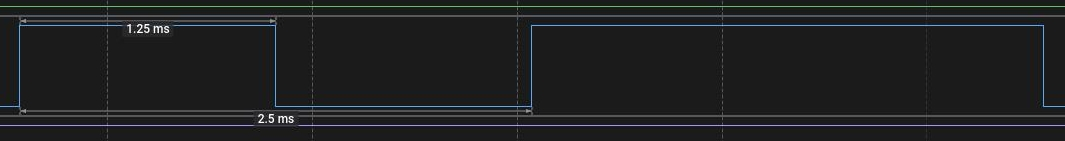
\includegraphics[width=0.7\textwidth]{../img/120rpm_to60_1.jpg}
	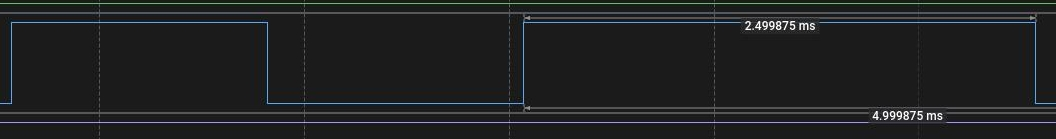
\includegraphics[width=0.7\textwidth]{../img/120rpm_to60_2.jpg}
	\caption[Moment of change between commands with 120RPM and 60RPM]{Moment of change between commands (120RPM $\Rightarrow$  60RPM)}
	\label{fig:switching}
\end{figure}

An attempt was made to also measure the delay  between switching commands, displayed in figure \ref{fig:switching}.
The results indicate that the delay between commands is imperceptible.
Similar outcomes were also observed for other command combinations.

This demonstrates the efficiency of the HAL layer in managing stepper motor control and transitioning seamlessly between commands.
As long as stepper queues are supplied with commands in advance, the platform can operate without noticeable interruptions.
Most importantly, the platform’s timely and predictable behavior ensures that mathematical corrections to the radar data can be applied accurately.

\section{MATLAB Control Interface}

In its basic operating mode the platform control is totally deattached from the radar system.
Radar data processing might do some correction based on the platform speed, accelerations and position but it doesn't send any commands to the platform itself.
Thus the control flow of the platform is rather simple -- user uploads a program to the microcontroller and starts it's execution.
In order to managed programs and provide window to read platform diagnostics from a simple MATLAB application was created.

\begin{figure}[h!]
	\centering
	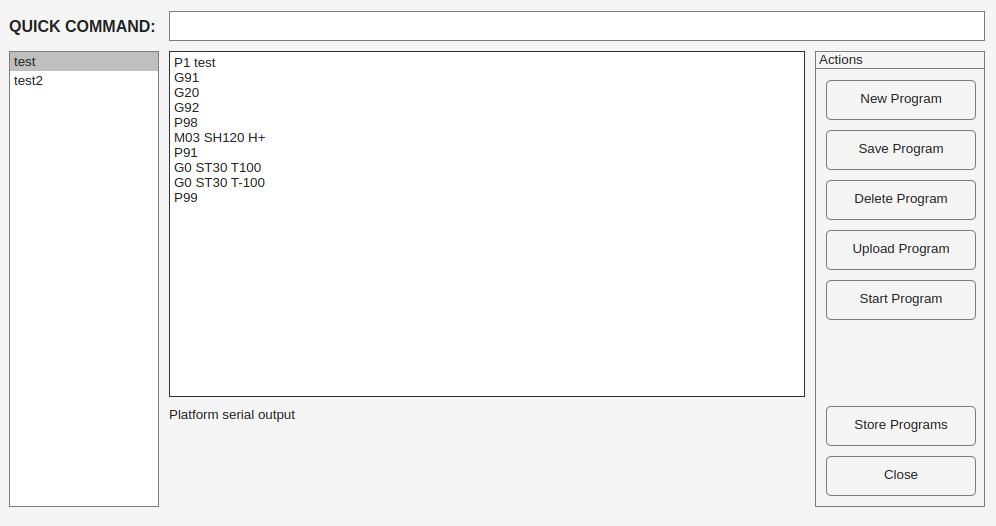
\includegraphics[width=0.9\textwidth]{../img/platform_control.jpg}
	\caption[GUI of the platform control]{GUI of the platform control}
	\label{fig:platformControl}
\end{figure}

After connecting to the platform (Picking correct port and baudrate in preferences, clicking the connect button in the main window.) user can go into platform control window \ref{fig:platformControl}.
On the left there is a sidebar with a list of all stored programs.
Clicking on any of them will load it into the editor windows and by presssing buttons on the right user can send the program to the platform.

After the program has been sent it can be either started manually by sending a start command from the \verb|QUICK COMMAND| box or by pressing the start button.
Using the start button will make sure that the platform queues are empty, the platform is homed and only then the program will start.
To see feedback from the platform user can see the text window on the bottom of the screen.



\chapter{Radar Data Processing}

\boldred{TODO: target detection at least using CFAR}

% vim.ft=tex
\chapter*{Conclusion}
\addcontentsline{toc}{chapter}{Conclusion}

TODO


%%% Bibliography (literature used as a source)
%%%
%%% We employ biblatex to construct the bibliography. It processes
%%% citations in the text (e.g., the \cite{...} macro) and looks up
%%% relevant entries in the bibliography.bib file.
%%%
%%% See also biblatex settings in thesis.tex.

%%% Generate the bibliography. Beware that if you cited no works,
%%% the empty list will be omitted completely.

% We let bibliography items stick out of the right margin a little
\def\bibfont{\hfuzz=2pt}

\printbibliography[heading=bibintoc]

%%% If case you prefer to write the bibliography manually (without biblatex),
%%% you can use the following. Please follow the ISO 690 standard and
%%% citation conventions of your field of research.

% \begin{thebibliography}{99}
%
% \bibitem{lamport94}
%   {\sc Lamport,} Leslie.
%   \emph{\LaTeX: A Document Preparation System}.
%   2nd edition.
%   Massachusetts: Addison Wesley, 1994.
%   ISBN 0-201-52983-1.
%
% \end{thebibliography}


\listoffigures

\listoftables

\clearpage
\openright
\end{document}

